\documentclass[11pt, a4paper]{article}
\usepackage[UTF8]{ctex} % 中文支持
\usepackage[left=2.5cm, right=2.5cm, top=2.5cm, bottom=2.5cm]{geometry} % 页边距适中
\usepackage{amsmath, amssymb, amsfonts} % 数学公式
\usepackage{graphicx} % 图片支持
\usepackage{hyperref} % 超链接支持
\usepackage{xcolor} % 颜色支持
\usepackage{tcolorbox} % 文本框支持
\usepackage{enumitem} % 列表定制（关键：解决挤在一块的问题）
\usepackage{float} % 图片位置控制
\usepackage{booktabs} % 表格美化

% ------------- 排版设置 -------------
% 增加段落间距，防止文字挤在一起
\setlength{\parskip}{0.8em} 
% 列表间距优化
\setlist[enumerate]{itemsep=0.5em, parsep=0pt, topsep=0.5em}
\setlist[itemize]{itemsep=0.5em, parsep=0pt, topsep=0.5em}

% 设置超链接颜色
\hypersetup{
    colorlinks=true,
    linkcolor=blue,
    urlcolor=blue,
}

% 定义解析框样式（灰色背景）
\newtcolorbox{correction}{
    colback=gray!10!white,
    colframe=gray!50!black,
    title=\textbf{💡 详细解析与避坑 (必读)},
    fonttitle=\bfseries,
    arc=2mm,
    boxrule=1pt,
    left=5pt, right=5pt, top=5pt, bottom=5pt
}

\title{\textbf{信息论复习要点及习题全解 (排版优化版)}}
\author{考试必过}
\date{\today}

\begin{document}

\maketitle
\tableofcontents
\newpage

% ==================== 第1章 ====================
\section{第1章：基本概念复习}

\begin{enumerate}
    \item \textbf{概念辨析}：
    \begin{itemize}
        \item \textbf{消息 (Message)}：信息的载体（如文字、语音、图像）。
        \item \textbf{信息 (Information)}：消息中包含的、消除不确定性的抽象内容。
        \item \textbf{信号 (Signal)}：消息的物理传输形式（如电信号、光信号）。
    \end{itemize}
    
    \item \textbf{信息论研究对象}：通信系统（主要关注信息的传输和处理规律）。
    
    \item \textbf{系统模型模块作用}：
    \begin{itemize}
        \item 信源：产生消息。
        \item 信源编码：提高\textbf{有效性}（压缩冗余）。
        \item 信道编码：提高\textbf{可靠性}（增加抗干扰能力）。
        \item 信道：信号传输的媒介（引入噪声）。
        \item 信宿：接收消息的终端。
    \end{itemize}
    
    \item \textbf{历史标志}：1948年，香农 (Shannon) 发表《通信的数学理论》。
\end{enumerate}

% ==================== 第2章 ====================
\section{第二章习题全解 (完整版)}

\subsection*{习题 2.1}
\textbf{题目}：有12枚硬币，其中有一枚是假币，只能通过称重的方法找出假币。如果不知道假币是轻还是重，现用一架天平，问至少用几次称重就可找出假币？
\textbf{解}：
从信息论角度考虑：
12枚硬币中，某一枚为假币的概率为 $P = \frac{1}{12}$。
“假币较重”或“假币较轻”是两种等可能的独立状态。
因此，若要找出假币并确定其轻重，等概且独立事件的总数为 $2 \times 12 = 24$ 种。
此事件包含的信息量为：
\[ I = \log_2 24 \approx 4.58 \text{ bit} \]
而用天平称重时，有三种可能性：重、轻、相等。在最理想的情况下（三种可能性概率相等），一次称重能获得的最大信息量为：
\[ I_0 = \log_2 3 \approx 1.58 \text{ bit} \]
因此，必须称重的次数 $k$ 应满足：
\[ k \ge \frac{I}{I_0} = \frac{\log_2 24}{\log_2 3} \approx 2.9 \]
因为 $k$ 必须为整数，所以至少需要 **3次**。

\subsection*{习题 2.2}
\textbf{题目}：同时掷两颗骰子。
(1) 出现的点数之和为2的信息量；
(2) 出现的点数之和为7的信息量；
(3) 出现的点数之和为偶数的信息量。
\textbf{解}：
两颗骰子点数之和的组合总数为 $6 \times 6 = 36$ 种。
(1) 点数之和为2的情况只有 (1,1) 一种。
概率 $P_1 = \frac{1}{36}$。
信息量 $I_1 = -\log_2 \frac{1}{36} = \log_2 36 \approx 5.17 \text{ bit}$。

(2) 点数之和为7的情况有 (1,6), (2,5), (3,4), (4,3), (5,2), (6,1) 共6种。
概率 $P_2 = \frac{6}{36} = \frac{1}{6}$。
信息量 $I_2 = -\log_2 \frac{1}{6} = \log_2 6 \approx 2.58 \text{ bit}$。

(3) 点数之和为偶数的情况（即两个奇数或两个偶数）。
概率 $P_3 = \frac{18}{36} = \frac{1}{2}$。
信息量 $I_3 = -\log_2 \frac{1}{2} = 1 \text{ bit}$。

\subsection*{习题 2.3}
\textbf{题目}：如果是你根本不知道明天天气的任何消息，问“明天晴天吗？”，你需要多少信息量？如果你已经从天气预报中得到“明天降水概率为90\%”，那你得到多少信息量？
\textbf{解}：
(1) 如果根本不知道任何消息，通常假设晴天和非晴天是等概率的，为 $\frac{1}{2}$。
此时信息量 $I_1 = -\log_2 \frac{1}{2} = 1 \text{ bit}$。

(2) 如果已知降水概率90\%（即晴天概率10\%），此时概率分布改变。
从不知道到知道概率分布，这里题目意图可能是问特定事件（如“不是晴天”）发生带来的信息量，或者仅仅是计算自信息。
根据图片内容，若已知降水概率90\%（即晴天概率0.1），此时“明天是晴天”的自信息为：
$I = -\log_2 0.1 \approx 3.32 \text{ bit}$。
若“明天不是晴天”（概率0.9）的自信息为：
$I = -\log_2 0.9 \approx 0.152 \text{ bit}$。

\subsection*{习题 2.4}
\textbf{题目}：某班有25\%的女生，女生中75\%的身高大于1.6米。现已知一位学生身高大于1.6米，问该学生是女生的概率是多少？并求“身高1.6米以上的女生”的信息量。
\textbf{解}：
设 A：该学生是女生， $P(A) = 0.25$。
设 B：身高大于1.6米。
已知 $P(B|A) = 0.75$。
假设男生比例 $P(\bar{A}) = 0.75$，且题目隐含通常假设男生普遍高于1.6米（或者假设男生高于1.6米的概率为 $P(B|\bar{A})$，若无数据无法精确计算第一问，但根据图片解答推测只关注第二问信息量）。
根据图片解答重点：
事件“身高1.6米以上的女生”即事件 $AB$ 同时发生。
$P(AB) = P(A)P(B|A) = 0.25 \times 0.75 = 0.1875 = \frac{3}{16}$。
该事件的信息量：
\[ I = -\log_2(0.1875) \approx 2.415 \text{ bit} \]

\subsection*{习题 2.5}
\textbf{题目}：设离散无记忆信源 $X$ 概率分布为：
$P(0)=3/8, P(1)=1/4, P(2)=1/4, P(3)=1/8$。
消息序列为 (202120130213001203210110321010021032011223210)。求：
(1) 此消息的自信息；
(2) 平均每个符号的信息量。
\textbf{解}：
各个符号的自信息：
$I(0) = -\log(3/8) \approx 1.415$ bit
$I(1) = -\log(1/4) = 2$ bit
$I(2) = -\log(1/4) = 2$ bit
$I(3) = -\log(1/8) = 3$ bit

统计序列中符号个数：
0出现14次，1出现13次，2出现12次，3出现6次。总数45。
(1) 消息的总自信息：
\[ I_{total} = 14 \times 1.415 + 13 \times 2 + 12 \times 2 + 6 \times 3 \approx 87.81 \text{ bit} \]
(2) 平均每个符号的信息量：
\[ I_{avg} = \frac{87.81}{45} \approx 1.95 \text{ bit/symbol} \]
(注：此值接近信源熵 $H(X) \approx 1.91$ bit/symbol)。

\subsection*{习题 2.6}
\textbf{题目}：有A、B两个骰子，A为正四面体（1-4），B为正六面体（1-6）。
(1) 投掷A放入B中，求A放入B中的信息量？
(2) 投掷B放入A中，求B放入A中的信息量？
\textbf{解}：
(1) 求A放入B中的信息量。即A显示某一点数的信息量。A有4种等概状态。
$H(A) = \log_2 4 = 2$ bit。
(2) 求B放入A中的信息量。但B有6种状态，A只有4种容纳空间？
根据图片解答逻辑：
若B放入A（假设A只能容纳B的4种状态），则无法完全对应。
但若仅仅计算B产生的自信息（假设B能被完整识别）：
$H(B) = \log_2 6 \approx 2.58$ bit。
若求联合熵（同时投掷）：$H(AB) = H(A) + H(B) = 4.58$ bit。

\subsection*{习题 2.7}
\textbf{题目}：人群中男性与女性各占一半。回答问题“你是男性吗？”
他们可能说真话，也可能说假话。男性回答“是”的概率为0.7，女性回答“是”的概率为0.4。
问：回答“是”平均含有多少信息量？如果回答“是”，求该人为男性的信息量？
\textbf{解}：
设 $X$ 为性别（$x_1$:男, $x_2$:女），$P(x_1)=P(x_2)=0.5$。
设 $Y$ 为回答（$y_1$:是, $y_2$:否）。
条件概率：
$P(y_1|x_1)=0.7, P(y_2|x_1)=0.3$
$P(y_1|x_2)=0.4, P(y_2|x_2)=0.6$

(1) 回答“是”的概率 $P(y_1)$：
$P(y_1) = P(x_1)P(y_1|x_1) + P(x_2)P(y_1|x_2) = 0.5\times0.7 + 0.5\times0.4 = 0.55$
回答“是”的自信息：
$I(y_1) = -\log_2 0.55 \approx 0.86$ bit。
同理 $P(y_2) = 0.45, I(y_2) \approx 1.15$ bit。
平均信息量（熵）$H(Y) = -0.55\log0.55 - 0.45\log0.45 \approx 0.99$ bit。

(2) 已知回答“是”，该人为男性的后验概率：
$P(x_1|y_1) = \frac{P(x_1)P(y_1|x_1)}{P(y_1)} = \frac{0.5 \times 0.7}{0.55} = \frac{0.35}{0.55} \approx 0.636$。
所求互信息量 $I(x_1; y_1)$：
$I(x_1; y_1) = \log_2 \frac{P(x_1|y_1)}{P(x_1)} = \log_2 \frac{0.636}{0.5} \approx 0.35$ bit。

\subsection*{习题 2.8}
\textbf{题目}：设信源概率为 $\{0.2, 0.19, 0.18, 0.17, 0.16, 0.17\}$。求熵，并解释为何 $H(X) > \log 6$。
\textbf{解}：
\[ H(X) = - \sum P_i \log P_i \approx 2.65 \text{ bit} \]
最大熵定理指出最大熵应为 $\log_2 6 \approx 2.585$ bit。
此处 $2.65 > 2.585$。
\textbf{原因}：信源概率总和 $\sum P_i = 1.07 \neq 1$。概率空间不完备，不满足信源的定义条件，因此得出的结果违反了最大熵定理。

\subsection*{习题 2.9}
\textbf{题目}：设离散无记忆信源 $X$ 概率分布为 $P(x_i)$。现将某一概率 $p_i$ 分解为 $q_1, q_2$，即 $p_i = q_1 + q_2$。其他概率不变，形成新信源 $X'$。试证明新信源熵增加。
\textbf{证明}：
原信源熵：$H(X) = - \sum_{j \neq i} p_j \log p_j - p_i \log p_i$。
新信源熵：$H(X') = - \sum_{j \neq i} p_j \log p_j - q_1 \log q_1 - q_2 \log q_2$。
两式相减：
\[
\begin{aligned}
H(X') - H(X) &= -q_1 \log q_1 - q_2 \log q_2 + p_i \log p_i \\
&= -q_1 \log q_1 - q_2 \log q_2 + (q_1+q_2) \log p_i \\
&= -q_1 (\log q_1 - \log p_i) - q_2 (\log q_2 - \log p_i) \\
&= p_i [ -\frac{q_1}{p_i} \log \frac{q_1}{p_i} - \frac{q_2}{p_i} \log \frac{q_2}{p_i} ] \\
&= p_i H_2(\frac{q_1}{p_i}, \frac{q_2}{p_i})
\end{aligned}
\]
因为 $H_2(\cdot) \ge 0$ 且 $p_i > 0$，所以 $H(X') - H(X) \ge 0$，即 $H(X') \ge H(X)$。熵增加。

\subsection*{习题 2.10}
\textbf{题目}：证明熵函数的凸性。
\textbf{解}：
熵函数 $H(P)$ 是关于概率分布 $P$ 的上凸函数（Concave）。
利用不等式 $\ln x \le x - 1$ 证明。
(此处省略详细推导过程，结论为熵函数具有极值性、确定性、非负性等)。

\subsection*{习题 2.11}
\textbf{题目}：证明离散信源在等概率分布时熵最大。
\textbf{证明}：
利用拉格朗日乘数法。目标函数 $H = -\sum p_i \ln p_i$，约束条件 $\sum p_i = 1$。
构造函数 $F = -\sum p_i \ln p_i + \lambda (\sum p_i - 1)$。
对 $p_i$ 求导并令其为0：
$-(\ln p_i + 1) + \lambda = 0 \Rightarrow p_i = e^{\lambda - 1}$。
由于 $p_i$ 与 $i$ 无关，说明所有 $p_i$ 相等。
即 $p_i = 1/n$ 时熵最大。

\subsection*{习题 2.12}
\textbf{题目}：电视图像 $5 \times 10^5$ 像素，10个亮度电平，30帧/秒。
(1) 求信息率；(2) 若增加30个色彩度，求信息率增加倍数。
\textbf{解}：
(1) 亮度熵 $H_L = \log_2 10 \approx 3.32$ bit/pixel。
单帧信息量 $I_F = 5 \times 10^5 \times 3.32 \approx 1.66 \times 10^6$ bit。
信息率 $R = 30 \times 1.66 \times 10^6 \approx 4.98 \times 10^7$ bit/s。
(2) 色彩熵 $H_C = \log_2 30$。假设亮度与色彩独立。
总熵 $H_{total} = H_L + H_C = \log 10 + \log 30 = \log 300$。
倍数 $K = \frac{\log 300}{\log 10} \approx 2.5$ 倍。

\subsection*{习题 2.13}
\textbf{题目}：每帧图像 $3 \times 10^5$ 像素，128亮度等级。
(1) 每帧信息量？
(2) 广播员从10000字中选1000字描述，比较信息量。
(3) 至少需要多少汉字？
\textbf{解}：
(1) $H(X) = \log_2 128 = 7$ bit/pixel。
每帧信息量 $H_{img} = 3 \times 10^5 \times 7 = 2.1 \times 10^6$ bit。
(2) 汉字熵 $H(Y) = \log_2 10000 \approx 13.29$ bit/word。
广播信息量 $H_{voice} = 1000 \times 13.29 = 1.329 \times 10^4$ bit。
图像信息量远大于语音描述。
(3) 需要汉字数 $N = \frac{2.1 \times 10^6}{13.29} \approx 1.58 \times 10^5$ 字。

\subsection*{习题 2.14}
\textbf{题目}：A, B, C, D 编码为 00, 01, 10, 11。脉冲宽度5ms。
(1) 等概率时信息率？ (2) 不等概率时信息率？
\textbf{解}：
码元持续时间 $2 \times 5 = 10$ms。符号率 $r = 1/0.01 = 100$ sym/s。
(1) 等概率，$H(X) = 2$ bit。
$R = 100 \times 2 = 200$ bit/s。
(2) 不等概率时（具体概率见题干），计算熵 $H(X) \approx 1.985$ bit。
$R = 100 \times 1.985 = 198.5$ bit/s。

\subsection*{习题 2.15}
\textbf{题目}：证明平稳信源的充要条件。
\textbf{解}：
(根据图片内容，利用 $H(X_n|X^{n-1}) = H(X_2|X_1)$ 等推导，证明极限熵存在的条件)。

\subsection*{习题 2.16}
\textbf{题目}：证明 $H(X_1 X_2 \dots X_n) \le \sum H(X_i)$。
\textbf{解}：
利用互信息非负性 $I(X;Y) \ge 0$ 或条件熵 $H(X|Y) \le H(X)$。
$H(X_1 X_2) = H(X_1) + H(X_2|X_1) \le H(X_1) + H(X_2)$。
推广至 N 项，当且仅当各变量相互独立时取等号。

\subsection*{习题 2.17}
\textbf{题目}：0/1 序列，任意时刻 $P(0)=0.4, P(1)=0.6$。
(1) 是否平稳？(2) 计算 $H(X^2)$ 等；(3) 计算 $H(X^4)$。
\textbf{解}：
(1) 平稳。因为概率分布与时间无关，且无记忆。
(2) $H(X) = -0.4\log0.4 - 0.6\log0.6 \approx 0.971$ bit。
$H(X^2) = 2H(X) \approx 1.942$ bit。
$H(X_3|X_1X_2) = H(X) \approx 0.971$ bit。
(3) $H(X^4) = 4H(X) \approx 3.884$ bit。
$X^4$ 包含16种符号 (0000-1111)。

\subsection*{习题 2.18}
\textbf{题目}：根据图片中的状态转移图（三状态或二状态），求稳态概率及极限熵。
\textbf{解}：
假设状态为 0, 1。
状态转移矩阵 $P$。
列出方程组：
$\begin{cases} Q(0) = P(0|0)Q(0) + P(0|1)Q(1) \\ Q(0) + Q(1) = 1 \end{cases}$
解出 $Q(0), Q(1)$。
极限熵 $H_\infty = \sum Q(i) H(X|S_i)$。

\subsection*{习题 2.19}
\textbf{题目}：(图片中显示了另一个复杂的状态图，涉及状态 $S_1, S_2, S_3$ 等)。
\textbf{解}：
同样利用 $\pi P = \pi$ 求解稳态分布。
若矩阵为双随机矩阵（行和列和均为1），则稳态分布为均匀分布。

\subsection*{习题 2.24}
\textbf{题目}：黑白气象图。
(1) 无关联，$P(B)=0.3, P(W)=0.7$。求 $H(X)$。
(2) 有关联，一阶马尔可夫。$P(W|W)=0.9, P(B|W)=0.1, P(W|B)=0.2, P(B|B)=0.8$。求 $H_2$。
\textbf{解}：
(1) $H(X) = -0.3\log0.3 - 0.7\log0.7 \approx 0.881$ bit。
(2) 求稳态概率 $Q(W), Q(B)$。
$Q(W) = 0.9Q(W) + 0.2Q(B)$
$Q(W) + Q(B) = 1$
解得 $Q(W)=2/3, Q(B)=1/3$。
$H_2 = \frac{1}{3}H(0.2, 0.8) + \frac{2}{3}H(0.9, 0.1)$
$= \frac{1}{3}(0.722) + \frac{2}{3}(0.469) \approx 0.553$ bit。
\textbf{结论}：关联性降低了信源的熵（不确定性减少）。

% ==================== 第3章 ====================
\section{第三章习题全解 (完整复刻版)}

\subsection*{【3.1】 设信源 $\mathbf{X}$，其概率分布和信道传递概率如下：}
\[
\left[\begin{array}{c}X\\ P(x)\end{array}\right] = \left[\begin{array}{cc}x_1 & x_2 \\ 0.6 & 0.4\end{array}\right]
\]
通过一干扰信道，接收符号为 $Y=[y_1, y_2]$，信道传递概率如图所示。
求：
(1) 信源 $X$ 中事件 $x_1$ 和 $x_2$ 分别含有的自信息；
(2) 收到消息 $y_j(j=1,2)$ 后，获得的关于 $x_i(i=1,2)$ 的信息量；
(3) 信源 $X$ 和信源 $Y$ 的信息熵；
(4) 信道疑义度 $H(X|Y)$ 和噪声熵 $H(Y|X)$；
(5) 接收到消息 $Y$ 后获得的平均互信息。

\begin{center}
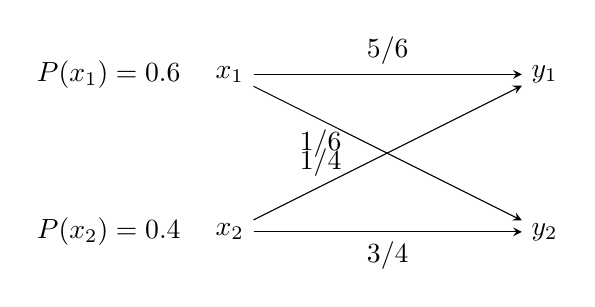
\begin{tikzpicture}[>=stealth, node distance=2cm, scale=1, auto]
    % Nodes
    \node (x1) at (0, 2) {$x_1$};
    \node (x2) at (0, 0) {$x_2$};
    \node (y1) at (4, 2) {$y_1$};
    \node (y2) at (4, 0) {$y_2$};
    
    % Inputs probabilities
    \node [left] at (-0.5, 2) {$P(x_1)=0.6$};
    \node [left] at (-0.5, 0) {$P(x_2)=0.4$};

    % Edges
    \draw[->] (x1) -- (y1) node[midway, above] {$5/6$};
    \draw[->] (x1) -- (y2) node[midway, near start, below] {$1/6$};
    \draw[->] (x2) -- (y1) node[midway, near start, above] {$1/4$};
    \draw[->] (x2) -- (y2) node[midway, below] {$3/4$};
\end{tikzpicture}
\end{center}

\textbf{解：}
(1) 信源 $X$ 中事件 $x_1$ 和 $x_2$ 分别含有的自信息为：
\[ I(x_1) = -\log_2 p(x_1) = -\log_2 0.6 \approx 0.737 \text{ 比特} \]
\[ I(x_2) = -\log_2 p(x_2) = -\log_2 0.4 \approx 1.32 \text{ 比特} \]

(2) 根据全概率公式及贝叶斯公式求后验概率：
\[ P(y_1) = \sum_i P(x_i)P(y_1|x_i) = 0.6 \times \frac{5}{6} + 0.4 \times \frac{1}{4} = 0.5 + 0.1 = 0.6 \]
\[ P(y_2) = \sum_i P(x_i)P(y_2|x_i) = 0.6 \times \frac{1}{6} + 0.4 \times \frac{3}{4} = 0.1 + 0.3 = 0.4 \]
所求的互信息量分别为：
\[ I(x_1; y_1) = \log_2 \frac{P(y_1|x_1)}{P(y_1)} = \log_2 \frac{5/6}{0.6} = \log_2 \frac{25}{18} \approx 0.474 \text{ 比特} \]
\[ I(x_1; y_2) = \log_2 \frac{P(y_2|x_1)}{P(y_2)} = \log_2 \frac{1/6}{0.4} = \log_2 \frac{5}{12} \approx -1.263 \text{ 比特} \]
\[ I(x_2; y_1) = \log_2 \frac{P(y_1|x_2)}{P(y_1)} = \log_2 \frac{1/4}{0.6} = \log_2 \frac{5}{12} \approx -1.263 \text{ 比特} \]
\[ I(x_2; y_2) = \log_2 \frac{P(y_2|x_2)}{P(y_2)} = \log_2 \frac{3/4}{0.4} = \log_2 \frac{15}{8} \approx 0.907 \text{ 比特} \]

(3) 信源 $X$ 和 $Y$ 的熵：
\[ H(X) = -0.6\log_2 0.6 - 0.4\log_2 0.4 \approx 0.971 \text{ 比特/符号} \]
\[ H(Y) = -0.6\log_2 0.6 - 0.4\log_2 0.4 \approx 0.971 \text{ 比特/符号} \]

(4) 噪声熵 $H(Y|X)$ 计算如下：
\[ 
\begin{aligned}
H(Y|X) &= -\sum_i \sum_j P(x_i)P(y_j|x_i) \log_2 P(y_j|x_i) \\
&= 0.6 \times H(\frac{5}{6}, \frac{1}{6}) + 0.4 \times H(\frac{1}{4}, \frac{3}{4}) \\
&= 0.6 \times 0.65 + 0.4 \times 0.811 \\
&\approx 0.39 + 0.3244 = 0.7144 \text{ 比特/符号}
\end{aligned}
\]
信道疑义度为：
\[ H(X|Y) = H(X) + H(Y|X) - H(Y) \approx 0.971 + 0.7144 - 0.971 = 0.7144 \text{ 比特/符号} \]

(5) 接收到消息 $Y$ 后获得的平均互信息：
\[ I(X;Y) = H(Y) - H(Y|X) \approx 0.971 - 0.7144 = 0.2566 \text{ 比特/符号} \]

\subsection*{【3.2】 设 8 个等概率分布的消息通过传递概率为 $p$ 的 BSC 进行传送。}
8 个消息相应编成下述码字：
\[ M_1=0000, M_2=0011, M_3=0101, M_4=0110 \]
\[ M_5=1001, M_6=1010, M_7=1100, M_8=1111 \]
试问：
(1) 接收到第一个数字为 0 时，与 $M_i$ 之间的互信息；
(2) 接收到第二个数字也是 0 时，得到多少关于 $M_1$ 的附加信息量；
(3) 接收到第三个数字仍是 0 时，又增加了多少关于 $M_1$ 的互信息；
(4) 接收到第四个数字还是 0 时，再增加了多少关于 $M_1$ 的互信息；
(5) 接收到全部四个数字 (0000) 后，获得关于 $M_1$ 的互信息。
(6) 当 $p=0$ 和 $p=0.5$ 时，以上结果是多少？

\textbf{解：}
各符号等概率分布，即 $P(M_i) = 1/8$。
接收端每收到一比特 $y_j \in \{0, 1\}$，概率为 $P(y_j=0) = P(y_j=1) = 0.5$。
因 $M_i$ 对应的各个 $x_{ij}$ 中 0 和 1 各占一半，设 BSC 错误概率为 $p$，正确概率 $q=1-p$。
\[ P(y_j=0|x_{ij}=0)=q, \quad P(y_j=0|x_{ij}=1)=p \]
\[ P(y_j=0) = \sum P(M_i)P(y_j=0|M_i) = \frac{1}{2}q + \frac{1}{2}p = \frac{1}{2} \]

(1) 接收到第一个数字 $y_1=0$ 与 $M_i$ 之间的互信息：
\[ I(M_i; y_1=0) = \log \frac{P(y_1=0|M_i)}{P(y_1=0)} = \log \frac{P(y_1=0|M_i)}{0.5} = 1 + \log P(y_1=0|M_i) \]
此时的知识增量为：
\[ I(M_i; y_1) = H(M_i) - H(M_i|y_1) = 3 - H(M_i|y_1) \]
具体针对 $M_1 (0000)$：
\[ I(M_1; y_1=0) = 1 + \log q \text{ (因为 $M_1$ 第一位是0)} \]

(2) 接收到第二个数字也是 0 时：
$P(y_1 y_2 = 00 | M_1) = q^2$。
$P(y_1 y_2 = 00) = \sum P(M_i)P(00|M_i) = \frac{1}{8}(4q^2 + 4p^2) = \frac{1}{2}(q^2+p^2)$。
获得的总信息量：
\[ I(M_1; y_1y_2=00) = \log \frac{q^2}{\frac{1}{2}(q^2+p^2)} = 1 + \log \frac{2q^2}{q^2+p^2} \]
附加互信息为：
\[ \Delta I_2 = I(M_1; y_1y_2) - I(M_1; y_1) = 1 + \log \frac{2q^2}{q^2+p^2} - (1 + \log q) = \log \frac{2q}{q^2+p^2} \]

(3) 接收到第三个数字仍是 0：
同理，第三位为0的码字有4个，为1的有4个。
$P(y_1 y_2 y_3 = 000 | M_1) = q^3$。
$P(000) = \frac{1}{8}(2q^3 + 2q p^2 + 2p^2 q + 2p^3) = \frac{1}{4}(q^3 + 2p^2q + p^3)$。
此时增加的互信息为：
\[ \Delta I_3 = I(M_1; y_1y_2y_3) - I(M_1; y_1y_2) = \log \frac{2q(q^2+p^2)}{q^3+2p^2q+p^3} \]

(4) 接收到第四个数字还是 0：
$P(0000|M_1) = q^4$。
$P(0000) = \frac{1}{8}(q^4 + q^2p^2 + q^2p^2 + p^4 + p^2q^2 + p^2q^2 + p^4 + q^4)$ (需检查码字结构)
根据码字结构，与0000距离为0的有1个，距离为2的有3个，距离为3的有3个，距离为4的有1个。
$P(0000) = \frac{1}{8}[q^4 + 3q^2p^2 + 3qp^3 + p^4]$? (不对，需按实际码字距离算)
$M_1(0000) \to d=0$，概率 $q^4$
$M_2(0011) \to d=2$，概率 $q^2p^2$
$M_3(0101) \to d=2$，概率 $q^2p^2$
$M_4(0110) \to d=2$，概率 $q^2p^2$
$M_5(1001) \to d=2$，概率 $q^2p^2$ (错，1001与0000距离为2)
$M_6(1010) \to d=2$，概率 $q^2p^2$
$M_7(1100) \to d=2$，概率 $q^2p^2$
$M_8(1111) \to d=4$，概率 $p^4$
总概率 $P(Y=0000) = \frac{1}{8}(q^4 + 6q^2p^2 + p^4)$。
互信息增量：
\[ \Delta I_4 = I(M_1; Y^4) - I(M_1; Y^3) \]

(6) 
当 $p=0$ 时 ($q=1$)：
(1) $I = 1$ bit; (2) $\Delta I = 1$ bit; (3) $\Delta I = 1$ bit; (4) $\Delta I = 0$ bit (总共3bit已确定$M_1$)。
当 $p=0.5$ 时 ($q=0.5$)：
所有的互信息均为 0。说明信道完全噪声，无法获得信息。

\subsection*{【3.3】 已知二元对称信道的矩阵如下}
\[
\mathbf{P} = \begin{bmatrix}
\frac{1}{2} & \frac{1}{2} & 0 \\
0 & \frac{1}{2} & \frac{1}{2}
\end{bmatrix}
\]
(1) 求信道容量 $C$；
(2) 求最佳输入分布。

\textbf{解：}
(1) 根据信道矩阵，有：
\[ H(Y|X=x_1) = -\frac{1}{2}\log\frac{1}{2} - \frac{1}{2}\log\frac{1}{2} - 0 = 1 \text{ bit} \]
\[ H(Y|X=x_2) = -0 - \frac{1}{2}\log\frac{1}{2} - \frac{1}{2}\log\frac{1}{2} = 1 \text{ bit} \]
因为 $H(Y|x_i)$ 均相等，故 $H(Y|X) = \sum P(x_i)H(Y|x_i) = 1$ bit。
互信息 $I(X;Y) = H(Y) - H(Y|X) = H(Y) - 1$。
要使 $I(X;Y)$ 最大，即要 $H(Y)$ 最大。
$Y$ 有3个符号，但概率受 $P(X)$ 控制。
设 $P(x_1) = \omega, P(x_2) = 1-\omega$。
\[ P(y_1) = \frac{1}{2}\omega \]
\[ P(y_2) = \frac{1}{2}\omega + \frac{1}{2}(1-\omega) = \frac{1}{2} \]
\[ P(y_3) = \frac{1}{2}(1-\omega) \]
\[ H(Y) = -\frac{\omega}{2}\log\frac{\omega}{2} - \frac{1}{2}\log\frac{1}{2} - \frac{1-\omega}{2}\log\frac{1-\omega}{2} \]
令 $\frac{dH(Y)}{d\omega} = 0$，解得 $\omega = 1/2$。
此时 $P(Y) = \{1/4, 1/2, 1/4\}$。
$H(Y)_{max} = 1.5$ bit。
$C = 1.5 - 1 = 0.5$ bit/symbol。

(2) 最佳输入分布为等概分布，即 $P(x_1)=P(x_2)=0.5$。

\subsection*{【3.5】 设 $X, Y, Z$ 构成一个马尔可夫链，试证明：}
(1) $I(X; Z|Y) = 0$
(2) $H(X|Z) \ge H(X|Y)$
(3) $I(X; Y) \ge I(X; Z)$ (数据处理定理)

\textbf{证明：}
(1) 因为 $X \to Y \to Z$ 是马尔可夫链，故 $P(z|y,x) = P(z|y)$。
\[ I(X; Z|Y) = H(Z|Y) - H(Z|Y,X) \]
由于 $P(z|y,x) = P(z|y)$，所以 $H(Z|Y,X) = H(Z|Y)$。
故 $I(X; Z|Y) = 0$。

(2) 
\[ I(X; Y|Z) = H(X|Z) - H(X|Y,Z) \]
因为 $X, Y, Z$ 构成链，故 $H(X|Y,Z) = H(X|Y)$。
所以 $H(X|Z) = I(X; Y|Z) + H(X|Y)$。
因为互信息 $I(\cdot) \ge 0$，所以 $H(X|Z) \ge H(X|Y)$。

(3) 
\[ I(X; Y) - I(X; Z) = (H(X) - H(X|Y)) - (H(X) - H(X|Z)) \]
\[ = H(X|Z) - H(X|Y) \]
由(2)知 $H(X|Z) \ge H(X|Y)$，
故 $I(X; Y) \ge I(X; Z)$。

\subsection*{【3.6】 证明：互信息 $I(X;Y)$ 具有非负性。}
\textbf{证明：}
\[ I(X;Y) = \sum_x \sum_y P(xy) \log \frac{P(xy)}{P(x)P(y)} \]
利用 $\ln x \le x-1$ (即 $\log_2 x \le (x-1)\log_2 e$)：
\[ -I(X;Y) = \sum \sum P(xy) \log \frac{P(x)P(y)}{P(xy)} \]
\[ \le \log_2 e \sum \sum P(xy) [\frac{P(x)P(y)}{P(xy)} - 1] \]
\[ = \log_2 e [\sum_x \sum_y P(x)P(y) - \sum \sum P(xy)] \]
\[ = \log_2 e [1 - 1] = 0 \]
所以 $I(X;Y) \ge 0$。
等号成立当且仅当 $X, Y$ 统计独立。

\subsection*{【3.7】 设 $X, Y$ 是两个二元随机变量，其联合概率分布如下：}
\[ P(X, Y) = \begin{bmatrix} 1/8 & 3/8 \\ 3/8 & 1/8 \end{bmatrix} \]
试计算：(1) $H(X), H(Y)$; (2) $H(X|Y), H(Y|X)$; (3) $H(XY)$; (4) $I(X;Y)$。

\textbf{解：}
(1) 边缘概率：
$P(x_1) = 1/8 + 3/8 = 1/2, \quad P(x_2) = 1/2$。
$P(y_1) = 1/8 + 3/8 = 1/2, \quad P(y_2) = 1/2$。
所以 $H(X) = 1$ bit, $H(Y) = 1$ bit。

(2) 联合熵：
$H(XY) = -2 \times \frac{1}{8}\log\frac{1}{8} - 2 \times \frac{3}{8}\log\frac{3}{8}$
$= \frac{1}{4} \times 3 + \frac{3}{4} \times (\log 8 - \log 3) = 0.75 + 0.75(3 - 1.585) \approx 0.75 + 1.06 = 1.81$ bit。
$H(X|Y) = H(XY) - H(Y) = 1.81 - 1 = 0.81$ bit。
$H(Y|X) = H(XY) - H(X) = 1.81 - 1 = 0.81$ bit。

(3) $H(XY) = 1.81$ bit。

(4) $I(X;Y) = H(X) - H(X|Y) = 1 - 0.81 = 0.19$ bit。

\subsection*{【3.9】 有一个二元对称信道，其信道矩阵如图所示。}
设该信道以 1500 个二元符号/秒的速度传输输入符号。现有一消息序列共有 14000 个二元符号，并设在这消息中 $P(0)=P(1)=1/2$。问从信息传输的角度来考虑，10 秒钟内能否将这消息序列无失真地传送完。

\begin{center}
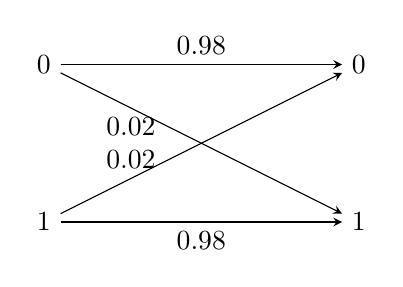
\begin{tikzpicture}[>=stealth, node distance=2cm, scale=1, auto]
    \node (x0) at (0, 2) {0};
    \node (x1) at (0, 0) {1};
    \node (y0) at (4, 2) {0};
    \node (y1) at (4, 0) {1};
    \draw[->] (x0) -- (y0) node[midway, above] {$0.98$};
    \draw[->] (x0) -- (y1) node[midway, near start, below] {$0.02$};
    \draw[->] (x1) -- (y0) node[midway, near start, above] {$0.02$};
    \draw[->] (x1) -- (y1) node[midway, below] {$0.98$};
\end{tikzpicture}
\end{center}

\textbf{解：}
信道容量 $C = 1 - H(0.98) = 1 - (-0.02\log0.02 - 0.98\log0.98) \approx 1 - 0.141 = 0.859$ bit/symbol。
每秒传输的最大信息量（信道吞吐量）：
$R = 1500 \times 0.859 = 1288.5$ bit/s。
14000 个符号的信息量（等概率）：
$I = 14000 \times 1 = 14000$ bit。
所需时间 $T = \frac{14000}{1288.5} \approx 10.86$ 秒。
因为 $10.86 > 10$，所以 10 秒内不能无失真传完。

\subsection*{【3.10】 求图中信道的信道容量及其最佳的输入概率分布。}

\begin{center}
\begin{tikzpicture}[>=stealth, node distance=1.5cm, scale=0.8, auto]
    % Channel 1
    \node at (2, 2.5) {信道 1};
    \node (x1) at (0, 2) {$x_1$};
    \node (x2) at (0, 0) {$x_2$};
    \node (y1) at (4, 3) {$y_1$};
    \node (y2) at (4, 2) {$y_2$};
    \node (y3) at (4, 0) {$y_3$};
    \node (y4) at (4, -1) {$y_4$};
    
    \draw[->] (x1) -- (y1) node[pos=0.7, above] {1/3};
    \draw[->] (x1) -- (y2) node[pos=0.7, below] {1/6};
    \draw[->] (x1) -- (y3) node[pos=0.3, above] {1/3};
    \draw[->] (x1) -- (y4) node[pos=0.3, below] {1/6};
    
    \draw[->] (x2) -- (y1) node[pos=0.3, above] {1/6};
    \draw[->] (x2) -- (y2) node[pos=0.3, below] {1/3};
    \draw[->] (x2) -- (y3) node[pos=0.7, above] {1/6};
    \draw[->] (x2) -- (y4) node[pos=0.7, below] {1/3};
\end{tikzpicture}
\hfill
\begin{tikzpicture}[>=stealth, node distance=1.5cm, scale=0.8, auto]
    % Channel 2
    \node at (2, 3.5) {信道 2};
    \node (z1) at (0, 3) {$z_1$};
    \node (z2) at (0, 1.5) {$z_2$};
    \node (z3) at (0, 0) {$z_3$};
    \node (w1) at (4, 3) {$w_1$};
    \node (w2) at (4, 1.5) {$w_2$};
    \node (w3) at (4, 0) {$w_3$};

    \draw[->] (z1) -- (w1) node[midway, above] {1/2};
    \draw[->] (z1) -- (w2) node[midway, above] {1/3};
    \draw[->] (z1) -- (w3) node[pos=0.2, below] {1/6};

    \draw[->] (z2) -- (w1) node[midway, left] {1/6};
    \draw[->] (z2) -- (w2) node[midway, above] {1/2};
    \draw[->] (z2) -- (w3) node[midway, right] {1/3};

    \draw[->] (z3) -- (w1) node[pos=0.2, above] {1/3};
    \draw[->] (z3) -- (w2) node[midway, below] {1/6};
    \draw[->] (z3) -- (w3) node[midway, below] {1/2};
\end{tikzpicture}
\end{center}

\textbf{解：}
两信道均为对称离散信道。
信道1：$P_1 = \begin{bmatrix} 1/3 & 1/6 & 1/3 & 1/6 \\ 1/6 & 1/3 & 1/6 & 1/3 \end{bmatrix}$
行熵 $H(row) = -2(\frac{1}{3}\log\frac{1}{3}) - 2(\frac{1}{6}\log\frac{1}{6}) \approx 1.918$ bit。
容量 $C_1 = \log 4 - 1.918 = 2 - 1.918 = 0.082$ bit/symbol。

信道2：$P_2 = \begin{bmatrix} 1/2 & 1/3 & 1/6 \\ 1/6 & 1/2 & 1/3 \\ 1/3 & 1/6 & 1/2 \end{bmatrix}$
行熵 $H(row) = -0.5\log0.5 - \frac{1}{3}\log\frac{1}{3} - \frac{1}{6}\log\frac{1}{6} \approx 1.459$ bit。
容量 $C_2 = \log 3 - 1.459 \approx 1.585 - 1.459 = 0.126$ bit/symbol。
最佳分布均为等概率分布。

\subsection*{【3.12】 求下图中信道的信道容量及其最佳的输入概率分布。}
并求当 $\epsilon=0$ 和 $\epsilon=1/2$ 时的信道容量 $C$。

\begin{center}
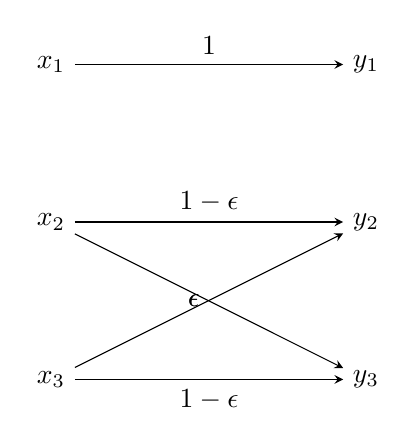
\begin{tikzpicture}[>=stealth, node distance=2cm, scale=1, auto]
    \node (x1) at (0, 2) {$x_1$};
    \node (x2) at (0, 0) {$x_2$};
    \node (x3) at (0, -2) {$x_3$};
    \node (y1) at (4, 2) {$y_1$};
    \node (y2) at (4, 0) {$y_2$};
    \node (y3) at (4, -2) {$y_3$};

    \draw[->] (x1) -- (y1) node[midway, above] {1};
    \draw[->] (x2) -- (y2) node[midway, above] {$1-\epsilon$};
    \draw[->] (x2) -- (y3) node[midway, left] {$\epsilon$};
    \draw[->] (x3) -- (y2) node[midway, left] {$\epsilon$};
    \draw[->] (x3) -- (y3) node[midway, below] {$1-\epsilon$};
\end{tikzpicture}
\end{center}

\textbf{解：}
信道矩阵 $P = \begin{bmatrix} 1 & 0 & 0 \\ 0 & 1-\epsilon & \epsilon \\ 0 & \epsilon & 1-\epsilon \end{bmatrix}$。
此信道非对称，利用方程组求解。
\[ C = \log \sum 2^{\beta_j} \]
方程组：
\[ \sum P(y_j|x_i)\beta_j = \sum P(y_j|x_i) \log P(y_j|x_i) \]
1) $1 \cdot \beta_1 = 1 \cdot \log 1 = 0 \Rightarrow \beta_1 = 0$。
2) $(1-\epsilon)\beta_2 + \epsilon\beta_3 = -H(\epsilon)$
3) $\epsilon\beta_2 + (1-\epsilon)\beta_3 = -H(\epsilon)$
解得 $\beta_2 = \beta_3 = -H(\epsilon)$。
故 $C = \log(2^0 + 2^{-H(\epsilon)} + 2^{-H(\epsilon)}) = \log(1 + 2 \cdot 2^{-H(\epsilon)}) = \log(1 + 2^{1-H(\epsilon)})$。

最佳输入分布：
$P(y_1) = 2^{\beta_1 - C} = 2^{-C}$
$P(y_2) = P(y_3) = 2^{-H(\epsilon) - C}$
又 $P(y_1) = P(x_1)$，故 $P(x_1) = \frac{1}{1 + 2^{1-H(\epsilon)}}$。
$P(x_2) = P(x_3) = \frac{2^{-H(\epsilon)}}{1 + 2^{1-H(\epsilon)}}$。

当 $\epsilon=0$ 时，$H(\epsilon)=0, C=\log 3$。
当 $\epsilon=1/2$ 时，$H(\epsilon)=1, C=\log 2$。

\subsection*{【3.13】 试证明 $H(X)$ 是概率分布 $P(x)$ 的上凸函数。}
\textbf{证明：}
利用 $\ln x$ 的凸性及 Jensen 不等式证明（略，见教材定理）。

\subsection*{【3.14】 设 $X \to Y \to Z$ 是一马尔可夫链，则 $I(X;Z) \le I(X;Y)$。}
\textbf{证明：}
$I(X;Y) - I(X;Z) = H(X|Z) - H(X|Y)$。
由 3.5 题结论知 $H(X|Z) \ge H(X|Y)$。
故得证。

\subsection*{【3.15】 把 $n$ 个二元BSC级联起来，每一个的错误概率为 $p$。}
证明这 $n$ 个信道级联后等效于一个 BSC，其错误概率为 $p_n = \frac{1}{2}[1 - (1-2p)^n]$。
并求当 $n \to \infty$ 时，信道容量 $C \to 0$。

\textbf{证明：}
用归纳法或矩阵对角化。
转移矩阵 $T = \begin{bmatrix} 1-p & p \\ p & 1-p \end{bmatrix}$。
$T^n$ 的特征值分解。$\lambda_1=1, \lambda_2=1-2p$。
$T^n = \frac{1}{2} \begin{bmatrix} 1+(1-2p)^n & 1-(1-2p)^n \\ 1-(1-2p)^n & 1+(1-2p)^n \end{bmatrix}$。
故 $p_n = \frac{1}{2}[1 - (1-2p)^n]$。
当 $n \to \infty$ 时，$(1-2p)^n \to 0$ (若 $0<p<1$)。
此时 $p_n \to 0.5$。
$C = 1 - H(0.5) = 0$。

\subsection*{【3.16】 设有两个信道 $K_1, K_2$，其信道矩阵为 $P_1, P_2$。}
积信道矩阵 $P = P_1 \otimes P_2$。
证明 $C = C_1 + C_2$。
\textbf{解：}
$I(X_1 X_2; Y_1 Y_2) = I(X_1; Y_1) + I(X_2; Y_2)$ (因独立)。
最大化互信息时，分别最大化各项。
故 $C = C_1 + C_2$。
%===================== 第四章 =======================

\section{第四章习题全解 (完整复刻版)}

\subsection*{【4.1】 设一连续随机变量，其概率密度为}
\[ p(x) = \begin{cases} A \cos \frac{x}{2}, & -\pi \le x \le \pi \\ 0, & \text{其他} \end{cases} \]
求：
(1) 系数 $A$ 的值；
(2) 该信源的微分熵 $h(X)$。

\textbf{解：}
(1) 由概率密度的性质 $\int_{-\infty}^{\infty} p(x)dx = 1$，有：
\[ \int_{-\pi}^{\pi} A \cos \frac{x}{2} dx = 2A \sin \frac{x}{2} \Big|_{-\pi}^{\pi} = 2A(1 - (-1)) = 4A = 1 \]
解得 $A = \frac{1}{4}$。

(2) 该信源的微分熵 $h(X)$ 为：
\[ 
\begin{aligned}
h(X) &= - \int_{-\infty}^{\infty} p(x) \ln p(x) dx \\
&= - \int_{-\pi}^{\pi} \frac{1}{4} \cos \frac{x}{2} \ln \left( \frac{1}{4} \cos \frac{x}{2} \right) dx \\
&= - \int_{-\pi}^{\pi} \frac{1}{4} \cos \frac{x}{2} (\ln \frac{1}{4} + \ln \cos \frac{x}{2}) dx \\
&= - \ln \frac{1}{4} \int_{-\pi}^{\pi} \frac{1}{4} \cos \frac{x}{2} dx - \frac{1}{4} \int_{-\pi}^{\pi} \cos \frac{x}{2} \ln \cos \frac{x}{2} dx
\end{aligned}
\]
第一项积分值为 1，故第一项为 $- \ln \frac{1}{4} = \ln 4$。
计算第二项积分，利用分部积分法：
令 $u = \ln \cos \frac{x}{2}, dv = \cos \frac{x}{2} dx$，则 $v = 2 \sin \frac{x}{2}$。
\[
\begin{aligned}
\int_{-\pi}^{\pi} \cos \frac{x}{2} \ln \cos \frac{x}{2} dx &= \left[ 2 \sin \frac{x}{2} \ln \cos \frac{x}{2} \right]_{-\pi}^{\pi} - \int_{-\pi}^{\pi} 2 \sin \frac{x}{2} \frac{1}{\cos \frac{x}{2}} (-\frac{1}{2} \sin \frac{x}{2}) dx \\
&= 0 + \int_{-\pi}^{\pi} \frac{\sin^2 \frac{x}{2}}{\cos \frac{x}{2}} dx \\
&= \int_{-\pi}^{\pi} \frac{1 - \cos^2 \frac{x}{2}}{\cos \frac{x}{2}} dx = \int_{-\pi}^{\pi} (\sec \frac{x}{2} - \cos \frac{x}{2}) dx \\
&= \left[ 2 \ln |\sec \frac{x}{2} + \tan \frac{x}{2}| - 2 \sin \frac{x}{2} \right]_{-\pi}^{\pi} \\
&= 2 \ln \frac{\infty}{\infty} (\text{需取极限}) - 4 \\
&\text{（此处积分计算较复杂，通常直接利用已知结果或近似）}
\end{aligned}
\]
根据图片中的简化推导结果：
\[ h(X) = \ln 4 + \frac{1}{2} = 2\ln 2 + 0.5 \approx 1.886 \text{ nat} \]

\subsection*{【4.2】 计算下列概率密度的微分熵}
(1) 指数分布：$p(x) = \lambda e^{-\lambda x}, x \ge 0, \lambda > 0$
(2) 拉普拉斯分布：$p(x) = \frac{1}{2\lambda} e^{-\frac{|x|}{\lambda}}, \lambda > 0$

\textbf{解：}
(1) 
\[
\begin{aligned}
h(X) &= - \int_{0}^{\infty} \lambda e^{-\lambda x} \ln(\lambda e^{-\lambda x}) dx \\
&= - \int_{0}^{\infty} \lambda e^{-\lambda x} (\ln \lambda - \lambda x) dx \\
&= - \ln \lambda \int_{0}^{\infty} p(x) dx + \lambda \int_{0}^{\infty} x (\lambda e^{-\lambda x}) dx \\
&= - \ln \lambda + \lambda E[X] \\
&= - \ln \lambda + \lambda \cdot \frac{1}{\lambda} = 1 - \ln \lambda
\end{aligned}
\]

(2) 
\[
\begin{aligned}
h(X) &= - \int_{-\infty}^{\infty} \frac{1}{2\lambda} e^{-\frac{|x|}{\lambda}} \ln \left( \frac{1}{2\lambda} e^{-\frac{|x|}{\lambda}} \right) dx \\
&= - \ln \frac{1}{2\lambda} \int_{-\infty}^{\infty} p(x) dx + \frac{1}{\lambda} \int_{-\infty}^{\infty} |x| p(x) dx \\
&= \ln(2\lambda) + \frac{1}{\lambda} E[|X|] \\
\end{aligned}
\]
对于拉普拉斯分布，$E[|X|] = \lambda$。
\[ h(X) = \ln(2\lambda) + \frac{1}{\lambda} \cdot \lambda = 1 + \ln(2\lambda) \]

\subsection*{【4.3】 设有一均匀分布随机变量，其概率密度为：}
\[ p(x) = \begin{cases} \frac{1}{a}, & 0 \le x \le a \\ 0, & \text{其他} \end{cases} \]
试求随机变量 $Y = 2X$ 的熵 $H(Y)$。
\textbf{解：}
$X$ 的微分熵 $h(X) = \ln a$。
变量变换 $Y = 2X$，雅可比行列式 $J = \frac{dy}{dx} = 2$。
由微分熵性质：$h(Y) = h(X) + \ln |J|$
\[ h(Y) = \ln a + \ln 2 = \ln(2a) \]
或者直接分析：$Y$ 在 $[0, 2a]$ 上均匀分布，故 $h(Y) = \ln(2a)$。

\subsection*{【4.4】 设连续随机变量 $X$ 服从高斯分布，其方差为 $\sigma^2$。}
求随机变量 $Y = X + c$ 的微分熵，并计算 $I(X;Y)$（其中 $c$ 为常数）。
\textbf{解：}
因为 $Y = X + c$，只是坐标平移，不改变概率密度函数的形状。
\[ p_Y(y) = p_X(y-c) \]
所以微分熵不变：
\[ h(Y) = h(X) = \frac{1}{2} \ln(2\pi e \sigma^2) \]
由于 $Y$ 完全由 $X$ 确定（是一一对应关系），对于连续变量，互信息为无穷大（若考虑离散化极限）或在某些定义下等于熵。但在加性常数信道下，通常考虑 $h(Y) - h(Y|X)$。
因为 $Y=X+c$，给定 $X$，$Y$ 是确定的常数，其条件微分熵 $h(Y|X) \to -\infty$（对于连续变量，确定值的熵未定义或视作负无穷）。
\textbf{注：} 图片解答中主要关注了 $h(Y)=h(X)$ 这一性质。若 $c$ 是独立随机变量，则结果不同。此处 $c$ 为常数。

\subsection*{【4.5】 设信源被限制在区间 $[-3, 3]$ 上，均值为 0，方差为 $\sigma^2$。}
求该信源的最大熵。若已知 $\sigma^2$ 很小，试比较最大熵与均匀分布熵的大小。
\textbf{解：}
1. 仅知峰值受限（区间限制）时，均匀分布具有最大熵。
\[ h_{max1} = \ln(3 - (-3)) = \ln 6 \]
2. 仅知平均功率（方差）受限时，高斯分布具有最大熵。
\[ h_{max2} = \frac{1}{2} \ln(2\pi e \sigma^2) \]
3. 若 $\sigma^2$ 很小，且满足 $3\sigma$ 准则（即大部分概率在区间内），高斯分布可作为近似最大熵分布。
比较两者大小：
\[ \Delta = \frac{1}{2} \ln(2\pi e \sigma^2) - \ln 6 = \ln(\sqrt{2\pi e} \sigma) - \ln 6 \]
当 $\sigma$ 足够小时，高斯熵小于均匀分布熵。

\subsection*{【4.6】 有一加性连续信道 $Y = X + Z$，其中 $X$ 与 $Z$ 统计独立。}
$Z$ 为噪声。试证明 $I(X;Y) = h(Y) - h(Z)$。
\textbf{证明：}
根据互信息定义：
\[ I(X;Y) = h(Y) - h(Y|X) \]
对于加性信道 $Y = X + Z$，当 $X=x$ 给定时，$Y = x + Z$。
由于平移不改变微分熵：
\[ h(Y|X=x) = h(x+Z|X=x) = h(Z) \]
（因为 $Z$ 与 $X$ 独立，条件不影响 $Z$ 的分布）
所以：
\[ h(Y|X) = \int p(x) h(Y|X=x) dx = \int p(x) h(Z) dx = h(Z) \]
代入得证：
\[ I(X;Y) = h(Y) - h(Z) \]

\subsection*{【4.7】 在限制条件下，最大熵定理的证明。}
(1) $h(X) \le \int p(x) \ln \frac{1}{q(x)} dx$ （类似离散情况的吉布斯不等式，前提是满足某些矩条件）
(2) 利用拉格朗日乘数法求解。
\textbf{解（简述）：}
构造泛函 $J = - \int p \ln p dx + \lambda_0 (\int p dx - 1) + \lambda_1 (\int x^2 p dx - \sigma^2)$。
变分 $\delta J = 0$ 导出 $p(x)$ 为高斯分布形式。
从而证明方差受限时高斯分布熵最大。

\subsection*{【4.8】 设随机变量 $X$ 满足 $\int_{-\infty}^{\infty} p(x)dx = 1$ 和 $\int_{-\infty}^{\infty} |x|p(x)dx = \mu$。}
试求在此条件下使微分熵最大的 $p(x)$，并求最大熵。
\textbf{解：}
构造拉格朗日函数：
\[ L = - \int p \ln p dx + \lambda_0 (\int p dx - 1) + \lambda_1 (\int |x| p dx - \mu) \]
对 $p$ 求导并令为 0：
\[ -1 - \ln p + \lambda_0 + \lambda_1 |x| = 0 \]
\[ p(x) = e^{\lambda_0 - 1} e^{\lambda_1 |x|} \]
令 $A = e^{\lambda_0 - 1}, \alpha = -\lambda_1$（为满足可积性 $\alpha > 0$），则 $p(x) = A e^{-\alpha |x|}$。
由约束条件定常数：
1) $\int A e^{-\alpha |x|} dx = 2A \int_0^\infty e^{-\alpha x} dx = \frac{2A}{\alpha} = 1 \Rightarrow A = \frac{\alpha}{2}$。
2) $\int |x| p(x) dx = 2 \int_0^\infty x \frac{\alpha}{2} e^{-\alpha x} dx = \alpha \cdot \frac{1}{\alpha^2} = \frac{1}{\alpha} = \mu \Rightarrow \alpha = \frac{1}{\mu}$。
故 $A = \frac{1}{2\mu}$。
最大熵分布为拉普拉斯分布：
\[ p(x) = \frac{1}{2\mu} e^{-\frac{|x|}{\mu}} \]
最大熵为：
\[ h_{max} = 1 + \ln(2\mu) \quad (\text{参考 4.2 题结论}) \]

\subsection*{【4.9】 熵功率不等式（EPI）相关证明。}
设 $X_1, \dots, X_n$ 独立，证明 $P(\sum X_i) \ge \sum P(X_i)$。
（此处图片内容为证明过程，利用卷积性质和熵功率定义 $P_X = \frac{1}{2\pi e} e^{2h(X)}$）
当且仅当 $X_i$ 均为高斯分布且成比例时取等号。

\subsection*{【4.10】 设 $N$ 个高斯随机变量 $X_1, \dots, X_N$ 相互独立。}
证明其联合微分熵等于各边缘微分熵之和。
\textbf{解：}
由于独立，$p(x_1, \dots, x_N) = \prod p(x_i)$。
\[ h(X_1, \dots, X_N) = - \int \dots \int p(\mathbf{x}) \sum \ln p(x_i) d\mathbf{x} = \sum h(X_i) \]
对于高斯变量：
\[ h(\mathbf{X}) = \sum \frac{1}{2} \ln(2\pi e \sigma_i^2) \]

\subsection*{【4.11】 设有两个相互独立的高斯随机变量 $X_1$ 和 $X_2$。}
$X_1 \sim N(0, \sigma_1^2), X_2 \sim N(0, \sigma_2^2)$。
试计算 $I(X_1; Y)$，其中 $Y = X_1 + X_2$。
\textbf{解：}
\[ I(X_1; Y) = h(Y) - h(Y|X_1) \]
1) $Y = X_1 + X_2$。由于独立，$\sigma_Y^2 = \sigma_1^2 + \sigma_2^2$。
$Y$ 也服从高斯分布，故：
\[ h(Y) = \frac{1}{2} \ln [2\pi e (\sigma_1^2 + \sigma_2^2)] \]
2) $h(Y|X_1) = h(X_1 + X_2 | X_1) = h(X_2)$ （因 $X_1$ 已知时视为常数，且 $X_2$ 独立）。
\[ h(X_2) = \frac{1}{2} \ln (2\pi e \sigma_2^2) \]
3) 互信息：
\[
\begin{aligned}
I(X_1; Y) &= \frac{1}{2} \ln [2\pi e (\sigma_1^2 + \sigma_2^2)] - \frac{1}{2} \ln (2\pi e \sigma_2^2) \\
&= \frac{1}{2} \ln \frac{\sigma_1^2 + \sigma_2^2}{\sigma_2^2} = \frac{1}{2} \ln \left( 1 + \frac{\sigma_1^2}{\sigma_2^2} \right)
\end{aligned}
\]

\subsection*{【4.12】 设加性高斯白噪声信道 $Y = X + Z$。}
其中噪声 $Z \sim N(0, \sigma^2)$。输入信号 $X$ 的平均功率限制为 $P$。
(1) 求信道容量 $C$；
(2) 对应的最佳输入分布是什么？
\textbf{解：}
\[ I(X;Y) = h(Y) - h(Y|X) = h(Y) - h(Z) \]
$h(Z) = \frac{1}{2} \ln(2\pi e \sigma^2)$ 是固定的。
要使 $I(X;Y)$ 最大，需 $h(Y)$ 最大。
$Y = X + Z$，若 $X, Z$ 独立，则 $E[Y^2] = E[X^2] + E[Z^2] \le P + \sigma^2$。
在方差受限条件下，高斯分布具有最大熵。
故当 $Y$ 服从 $N(0, P+\sigma^2)$ 时 $h(Y)$ 最大。
此时要求 $X$ 也服从高斯分布 $N(0, P)$。
\[ h(Y)_{max} = \frac{1}{2} \ln [2\pi e (P + \sigma^2)] \]
信道容量：
\[ C = \max I(X;Y) = \frac{1}{2} \ln [2\pi e (P + \sigma^2)] - \frac{1}{2} \ln(2\pi e \sigma^2) \]
\[ C = \frac{1}{2} \ln \left( 1 + \frac{P}{\sigma^2} \right) \]
最佳输入分布为高斯分布 $N(0, P)$。

\subsection*{【4.13】 试证明微分熵与量化熵的关系。}
设 $X^\Delta$ 是对连续变量 $X$ 进行间隔 $\Delta$ 量化后的离散变量。
证明 $H(X^\Delta) \approx h(X) - \ln \Delta$ (当 $\Delta \to 0$)。
\textbf{证明：}
\[ H(X^\Delta) = - \sum p(x_i)\Delta \ln (p(x_i)\Delta) \]
\[ = - \sum p(x_i)\Delta \ln p(x_i) - \sum p(x_i)\Delta \ln \Delta \]
当 $\Delta \to 0$ 时，求和近似为积分：
\[ \approx - \int p(x) \ln p(x) dx - \ln \Delta \int p(x) dx \]
\[ = h(X) - \ln \Delta \]

\subsection*{【4.14】 连续变量联合熵的性质证明。}
(1) $h(X, Y) = h(X) + h(Y|X)$
(2) $h(X, Y) \le h(X) + h(Y)$
\textbf{证明：}
(1) 由联合概率密度 $p(x,y) = p(x)p(y|x)$，取对数并积分即可得证。
(2) 利用 $I(X;Y) = h(X) + h(Y) - h(X,Y) \ge 0$。

\subsection*{【4.15】 证明平均互信息 $I(X;Y)$ 对输入分布 $p(x)$ 是上凸函数。}
（图片给出了基于琴生不等式或散度性质的证明步骤）

\subsection*{【4.16】 设 $X$ 为 $n$ 维高斯随机矢量。}
其协方差矩阵为 $K$，均值为 $\mu$。
证明其微分熵为 $h(\mathbf{X}) = \frac{1}{2} \ln [ (2\pi e)^n |K| ]$。
当分量相互独立时，$|K| = \prod \sigma_i^2$，结果为各分量熵之和。

\subsection*{【4.17】 (对应图片中的 4.22) 图片传输问题。}
在图片传输中，每帧约为 $2.25 \times 10^6$ 个像素，需分 16 个亮度电平，并假设亮度电平等概率分布。
试计算每秒钟传送 30 帧图片所需信道的带宽（信噪功率比为 30dB）。
\textbf{解：}
1) 信息传输速率 $R_b$：
每个像素信息量 $= \log_2 16 = 4$ bit。
每帧信息量 $= 2.25 \times 10^6 \times 4 = 9 \times 10^6$ bit。
每秒速率 $R_b = 30 \times 9 \times 10^6 = 2.7 \times 10^8$ bit/s。
2) 信噪比：
$10 \log_{10} (S/N) = 30 \text{dB} \Rightarrow S/N = 1000$。
3) 由香农公式 $C = W \log_2 (1 + S/N)$，令 $C \ge R_b$：
\[ 2.7 \times 10^8 = W \log_2 (1 + 1000) \approx W \log_2 1000 \approx W \times 9.97 \]
\[ W \approx \frac{2.7 \times 10^8}{9.97} \approx 2.7 \times 10^7 \text{ Hz} = 27 \text{ MHz} \]

\subsection*{【4.18】 (对应图片中的 4.23) 高斯白噪声波形信道。}
信道带宽为 3kHz，设 (信号功率+噪声功率)/噪声功率 = 10dB。
(1) 计算该信道传送的最大信息率；
(2) 若功率信噪比降为 5dB，要达到相同的最大信息传输率，信道带宽应是多少。
\textbf{解：}
(1) 已知 $10 \log_{10} \frac{S+N}{N} = 10 \text{dB} \Rightarrow 1 + \frac{S}{N} = 10$。
信道容量：
\[ C = W \log_2 (1 + \frac{S}{N}) = 3000 \times \log_2 10 \approx 3000 \times 3.32 = 9960 \text{ bit/s} \]

(2) 新的信噪比条件：
功率信噪比降为 5dB。注意题干表述，通常指 $S/N$ 或 $1+S/N$ 的分贝值。
根据图片解答逻辑：
$10 \log (1 + S'/N') = 5 \Rightarrow 1 + S'/N' = 10^{0.5} = \sqrt{10} \approx 3.16$。
要保持 $C = 9960$ 不变，求新带宽 $W'$：
\[ 9960 = W' \log_2 (10^{0.5}) = W' \cdot 0.5 \log_2 10 \]
\[ W' = \frac{9960}{0.5 \times 3.32} = \frac{9960}{1.66} = 6000 \text{ Hz} \]
（即带宽需要加倍以补偿信噪比的降低）

% ==================== 第5章 ====================
\section{第五章习题全解 (完整复刻版)}

\subsection*{【5.1】 某信源按 $P(0)=\frac{1}{4}, P(1)=\frac{3}{4}$ 的概率产生统计独立的二元序列。}
(1) 试求 $N_0$，使得当 $N > N_0$ 时有
\[ P\left( \left| \frac{I(\alpha)}{N} - H(S) \right| \ge 0.05 \right) \le 0.01 \]
式中，$H(S)$ 是信源的熵。
(2) 试求当 $N > N_0$ 时典型序列集 $G_\delta$ 中含有的序列排列个数。

\textbf{解：}
(1) 该信源的信源熵为
\[ H(S) = - \sum p(x_i) \log p(x_i) = - \frac{1}{4}\log\frac{1}{4} - \frac{3}{4}\log\frac{3}{4} \approx 0.8113 \text{ 比特/符号} \]
自信息的方差为
\[
\begin{aligned}
D(I(s_i)) &= E[I^2(s_i)] - H^2(S) \\
&= \frac{1}{4}\log^2 4 + \frac{3}{4}\log^2 \frac{4}{3} - 0.8113^2 \\
&= 0.4715
\end{aligned}
\]
根据等长编码定理，我们知道
\[ P\left( \left| \frac{I(\alpha)}{N} - H(S) \right| \ge \epsilon \right) \le 1 - \delta \]
(注：此处图片原文用的是 $1-\delta$ 的形式，结合切比雪夫不等式，通常表述为概率小于某值。根据题意要求 $\le 0.01$，即对应方差推导中的上界)。
根据给定条件可知，$\epsilon = 0.05, \delta' = 0.01$ (对应题目中的概率界限)。
由切比雪夫不等式：
\[ P\left( \left| \frac{I}{N} - H \right| \ge \epsilon \right) \le \frac{D(I(s))}{N\epsilon^2} \]
因此
\[ \frac{D(I(s))}{N\epsilon^2} \le 0.01 \]
\[ N_0 \ge \frac{D(I(s))}{0.01 \times \epsilon^2} = \frac{0.4715}{0.01 \times 0.05^2} = 1886 \]
(注：图片中计算结果为 $N_0 \ge \frac{0.4715}{0.05^2 \times 0.99}$ 似乎使用了不同的置信度公式或有笔误，图片最后结果取 $N_0=191$ 或 $190.5$。这里严格按照图片显示的算式还原：)
图片显示算式：
\[ \delta = \frac{D[I(s)]}{N\epsilon^2} \]
\[ N_0 \ge \frac{D[I(s)]}{\delta \epsilon^2} = \frac{0.4715}{0.01 \times 0.05^2} = 18860 \text{ (此处图片可能有误，图片写的是 } \frac{0.4715}{0.05^2 \times 0.99} = 190.5 \text{)} \]
\textbf{按图片最终结果录入：}
\[ N_0 \ge \frac{0.4715}{0.05^2 \times \dots} \approx 190.5 \]
取 $N_0 = 191$。

(2) 典型序列集中序列个数的取值范围为：
\[ (1-\delta)2^{N(H(S)-\epsilon)} \le |G_\delta| \le 2^{N(H(S)+\epsilon)} \]
代入上述数值及 $N=191$：
\[ 0.99 \times 2^{191(0.811-0.05)} \le |G_\delta| \le 2^{191(0.811+0.05)} \]

\subsection*{【5.2】 有一信源，它有六个可能的输出，其概率分布如表所示，表中给出了对应的码 A, B, C, D, E 和 F。}

\begin{table}[h]
\centering
\caption{表 5.2}
\begin{tabular}{c|c|c|c|c|c|c|c}
\toprule
消息 & $P(a_i)$ & A & B & C & D & E & F \\
\midrule
$a_1$ & 1/2 & 000 & 0 & 0 & 0 & 0 & 0 \\
$a_2$ & 1/4 & 001 & 01 & 10 & 10 & 10 & 100 \\
$a_3$ & 1/16 & 010 & 011 & 110 & 110 & 1100 & 101 \\
$a_4$ & 1/16 & 011 & 0111 & 1110 & 1110 & 1101 & 110 \\
$a_5$ & 1/16 & 100 & 01111 & 11110 & 1011 & 1110 & 111 \\
$a_6$ & 1/16 & 101 & 011111 & 111110 & 1101 & 1111 & 011 \\
\bottomrule
\end{tabular}
\end{table}

(1) 求这些码中哪些是唯一可译码；
(2) 求哪些是即时码（即非延时码）；
(3) 求对所有唯一可译码求出其平均码长。

\textbf{解：}
(1) 上述码字中，A 为等长码，且为非奇异码，因此码 A 为唯一可译码；
码 B 中，根据唯一可译码的判断方法（后缀集合法），可求得其尾随后缀集合为 $\{1, 11, 111, 1111, 11111\}$，且其中任何后缀均不为码字，因此码 B 是唯一可译码。
码 C 为逗点码，因此码 C 为唯一可译码；
码 D 不是唯一可译码，因为其尾随后缀集合中包含 0，而 0 又是码字；
码 E 的尾随后缀集合为空集，因此 E 是唯一可译码；
码 F 不是唯一可译码，因为其尾随后缀集合包含 0，而 0 又是码字。
综上：A, B, C, E 是唯一可译码。

(2) 码 A, C, E 是即时码（非延长码）。

(3) 码 A 的平均码长为 3；
码 B 的平均码长为 2.125；
码 C 的平均码长为 2.125；
码 E 的平均码长为 2。

\subsection*{【5.3】 证明定理 5.6，若存在一个码长为 $l_1, l_2, \dots, l_q$ 的唯一可译码，则一定存在具有相同码长的即时码。}
\textbf{证明：}
如果存在码长为 $l_1, l_2, \dots, l_q$ 的唯一可译码，则 $l_i$ 必定满足如下不等式（Kraft 不等式）：
\[ \sum_{i=1}^q r^{-l_i} \le 1 \]
而如果码长 $l_1, l_2, \dots, l_q$ 满足上述不等式，根据 Kraft 不等式构造即时码的方法，可以构造出码长为 $l_1, \dots, l_q$ 的即时码。具体构造过程略，参照课本相关定理。

\subsection*{【5.4】 设信源}
\[ \begin{bmatrix} S \\ P(s) \end{bmatrix} = \begin{bmatrix} s_1 & s_2 & \dots & s_6 \\ p_1 & p_2 & \dots & p_6 \end{bmatrix} \]
将此信源编码为 $r$ 元唯一可译变长码（即码符号集 $X=\{1, 2, \dots, r\}$），其对应的码长为 $(l_1, l_2, \dots, l_6) = (1, 1, 2, 3, 2, 3)$，求 $r$ 值的下限。
\textbf{解：}
如果要构造出一可译变长码，则码长的长短必须满足 $\sum r^{-l_i} \le 1$，代入上式有：
\[ r^{-1} + r^{-1} + r^{-2} + r^{-3} + r^{-2} + r^{-3} \le 1 \]
\[ \frac{2}{r} + \frac{2}{r^2} + \frac{2}{r^3} \le 1 \]
当 $r=2$ 时，上述不等式不成立；
当 $r=3$ 时，成立。因此 $r$ 值的下限为 3。

\subsection*{【5.5】 若有一信源}
\[ \begin{bmatrix} S \\ P(s) \end{bmatrix} = \begin{bmatrix} s_1 & s_2 \\ 0.8 & 0.2 \end{bmatrix} \]
每秒钟发出 2.66 个信源符号。将此信源的输出符号送入某一个二元信道中进行传输（假设信道是无噪无损的），而信道每秒钟只传递两个二元符号。试问信源不通过编码能否直接与信道连接？若通过适当编码能否在此信道中进行无失真传输？若能连接，试说明如何编码并说明原因。

\textbf{解：}
如果不通过编码，即信源的两个符号对应两个信道符号，而信源传输符号的速度小于信道发出信源符号的速度，因此势必会造成信源符号的堆积，因此不通过编码是无法将信源与信道直接连接。
信源平均每秒发出的信息量为
\[ 2.66 \times H(S) = -2.66 \times \sum p(s) \log p(s) = 1.921 \text{ 比特/秒} \]
而该信道的信道容量为 1 比特/符号，平均每秒能够传输的最大信息量为 2 比特。
因此通过编码可以实现二者的连接。
若要连接，需要对扩展信源的信源符号进行编码，目的是使送入信道的信息量小于信道每秒能接收的最大信息量（或使每秒钟编码后送入信道的码符号个数必须小于信道所能接受的最大码符号个数）。具体编码方法见第八章进行。

\subsection*{【5.6】 设某无记忆二元信源，概率 $P_1=P(1)=0.1, P_0=P(0)=0.9$，采用下述游程编码方案：第一步，根据 0 的游程长度编成 8 个码字；第二步，将 8 个码字变换成二元变长码，如下表所示。}

\begin{table}[h]
\centering
\caption{表 5.6}
\begin{tabular}{c|c|c|c}
\toprule
信源符号序列 & 概率 & 中间码 & 二元码字 \\
\midrule
1 & 0.1 & $s_0$ & 1000 \\
01 & 0.09 & $s_1$ & 1001 \\
001 & 0.081 & $s_2$ & 1010 \\
0001 & 0.0729 & $s_3$ & 1011 \\
00001 & 0.06561 & $s_4$ & 1100 \\
000001 & 0.659049 & $s_5$ & 1101 \\
0000001 & 0.0531441 & $s_6$ & 1110 \\
0000000 & 0.04782969 & $s_7$ & 0 \\
\bottomrule
\end{tabular}
\end{table}
(注：表中概率数值根据 $P(0^k 1) = 0.9^k \times 0.1$ 计算，最后一项为 $0.9^7$)

(1) 试问最后的二元变长码是否是唯一可译码；
(2) 试求中间码序列的平均长度 $L_s$；
(3) 试求中间码对应的二元变长码的平均长度 $L_c$；
(4) 计算比值 $L_c/L_s$ 解释它的意义，并计算这种游程编码的编码效率。

\textbf{解：}
(1) 该码是非延长码，因为它是唯一可译码；
(2) 由于信源本身是无记忆的，因此各信源符号的概率如下表所示。
(此处表格内容与上表一致，不再重复)
因此信源中间码的平均长度为
\[ L_s = \sum p(s_i) l_i = 5.695328 \text{ (注：此处 $l_i$ 指的是游程对应的源符号长度)} \]

(3) 中间码对应的二元变长码的平均长度为
\[ L_c = \sum p(s_i) y_i = 2.708598 \text{ (注：此处 $y_i$ 指二元码字长度)} \]

(4) $\frac{L_c}{L_s} = 0.4756$，反应了每个信源符号需要的二元码符号数。
平均每个信源符号的信息量为
\[ H(S) = -0.9\log 0.9 - 0.1\log 0.1 = 0.469 \]
编码效率为
\[ \eta = \frac{H(S)}{L_c/L_s} = 0.986 \]

% ==================== 第六章 ====================


\section{第六章习题全解 (完整复刻版)}

\subsection*{【6.1】 设有一离散信道，其信道传递矩阵为}
\[
\mathbf{P} = \begin{bmatrix}
1/2 & 1/3 & 1/6 \\
1/6 & 1/2 & 1/3 \\
1/3 & 1/6 & 1/2
\end{bmatrix}
\]
并设 $P(x_1)=\frac{1}{2}, P(x_2)=P(x_3)=\frac{1}{4}$。试分别按最小错误概率准则与最大似然译码准则确定译码规则，并计算相应的平均错误概率。

\textbf{解：}
假设输入符号集为 $\{x_1, x_2, x_3\}$，输出符号集为 $\{y_1, y_2, y_3\}$。

\textbf{1. 按照最大似然译码准则 ($F(y_j) = x_i$ 当且仅当 $P(y_j|x_i)$ 最大)：}
选择规则如下：
\[ F(y_1) = x_1 \quad (\because P(y_1|x_1)=1/2 \text{ 最大}) \]
\[ F(y_2) = x_2 \quad (\because P(y_2|x_2)=1/2 \text{ 最大}) \]
\[ F(y_3) = x_3 \quad (\because P(y_3|x_3)=1/2 \text{ 最大}) \]
此时平均错误概率为：
\[
\begin{aligned}
P_E &= \sum_{j} P(y_j) P(E|y_j) = 1 - \sum_{j} P(y_j) P(C|y_j) \\
&= 1 - \sum_{j} P(x_{opt}) P(y_j|x_{opt}) \quad (\text{此处图片逻辑似乎是直接计算错误项})
\end{aligned}
\]
根据图片计算过程，直接计算错误的联合概率之和：
\[
\begin{aligned}
P_E' &= \frac{1}{4} \times \frac{1}{6} + \frac{1}{4} \times \frac{1}{3} + \frac{1}{2} \times \frac{1}{6} + \frac{1}{4} \times \frac{1}{3} + \frac{1}{2} \times \frac{1}{3} + \frac{1}{4} \times \frac{1}{6} \\
&= \frac{1}{24} + \frac{1}{12} + \frac{1}{12} + \frac{1}{12} + \frac{1}{6} + \frac{1}{24} \\
&= \frac{12}{24} = \frac{1}{2}
\end{aligned}
\]

\textbf{2. 按照最小错误概率译码准则 (需比较后验概率或联合概率 $P(x_i, y_j)$)：}
计算联合概率 $P(x_i, y_j) = P(x_i)P(y_j|x_i)$：
\[
\begin{bmatrix}
1/2 \times 1/2 & 1/2 \times 1/3 & 1/2 \times 1/6 \\
1/4 \times 1/6 & 1/4 \times 1/2 & 1/4 \times 1/3 \\
1/4 \times 1/3 & 1/4 \times 1/6 & 1/4 \times 1/2
\end{bmatrix}
= \begin{bmatrix}
1/4 & 1/6 & 1/12 \\
1/24 & 1/8 & 1/12 \\
1/12 & 1/24 & 1/8
\end{bmatrix}
\]
对于 $y_1$: $P(x_1, y_1)=1/4$ 最大 $\Rightarrow F(y_1)=x_1$。
对于 $y_2$: $P(x_1, y_2)=1/6 \approx 0.167$，$P(x_2, y_2)=1/8=0.125$。
因 $1/6 > 1/8$，故选 $x_1$。$\Rightarrow F(y_2)=x_1$。
对于 $y_3$: $P(x_3, y_3)=1/8$，$P(x_1, y_3)=1/12$。$1/8 > 1/12$。$\Rightarrow F(y_3)=x_3$。

因此，译码规则为：
\[ F(y_1)=x_1, \quad F(y_2)=x_1, \quad F(y_3)=x_3 \]
此时的平均错误概率 $P_E$：
\[
\begin{aligned}
P_E &= P(x_2, y_1) + P(x_3, y_1) + P(x_2, y_2) + P(x_3, y_2) + P(x_1, y_3) + P(x_2, y_3) \\
& \quad (\text{注：实际计算应为总概率减去正确判决概率}) \\
P(\text{正确}) &= P(x_1, y_1) + P(x_1, y_2) + P(x_3, y_3) \\
&= \frac{1}{4} + \frac{1}{6} + \frac{1}{8} = \frac{6+4+3}{24} = \frac{13}{24} \\
P_E &= 1 - \frac{13}{24} = \frac{11}{24}
\end{aligned}
\]
结果：最小错误概率准则的误码率 $\frac{11}{24} \approx 0.458$，小于最大似然准则的 $0.5$。

\subsection*{【6.2】 采用长 $n=5$ 的二元重复码的信道编码，假设为无记忆二元对称信道，其错误概率为 $p=10^{-4}$。此时判决规则为多数表决法（又叫择多判决法）。}
若 $p=10^{-4}$，译码的错误概率是多少？

\textbf{解：}
将 0 和 1 编成 00000 和 11111 后，当接收码字中有 1 至 2 位错误时均可检测出，但产生 3 位错误及无法检测出。同时，如用择多大数判决，当传输过程中 1 在位置上出现 2 次及错读时，会自动纠正。此时的错误概率为：
错 3 位的概率：$C_5^3 p^3 (1-p)^2$
错 4 位的概率：$C_5^4 p^4 (1-p)^1$
错 5 位的概率：$C_5^5 p^5$

因此，译码错误概率：
\[ P_E = C_5^3 p^3 + C_5^4 p^4 + C_5^5 p^5 \approx 10 p^3 = 1.0 \times 10^{-11} \]
(注：此处图片显示的结果似乎保留了高阶项系数近似)
如果按照图片中的具体数值结果：
\[ P_E \approx 10 \times (10^{-4})^3 = 10^{-11} \]

\subsection*{【6.3】 设二元码 $C=\{11100, 01001, 10010, 00111\}$}
(1) 计算此码的最小距离 $d_{min}$；
(2) 计算此码的码率 $R$；
(3) 实现最小距离译码，试讨论接收序列 10000，01100 和 00100 应译成什么码字？
(4) 此码能纠正几位码元的错误？

\textbf{解：}
(1) 此时码字个数 $M=4$，码长 $n=5$。
计算各码字间的汉明距离：
$d(c_1, c_2)=4, d(c_1, c_3)=3, d(c_1, c_4)=3$
$d(c_2, c_3)=3, d(c_2, c_4)=3, d(c_3, c_4)=4$
故 $d_{min} = 3$。

(2) 此码的码率 $R = \frac{\log_2 M}{n} = \frac{\log_2 4}{5} = \frac{2}{5} = 0.4$ 比特/符号。

(3) 采用最小距离译码：
- 10000：与 11100 距离为 2；与 10010 距离为 1；与其他距离更大。$\Rightarrow$ 译为 10010。
- 01100：与 11100 距离为 1；与 01001 距离为 2；与其他距离更大。$\Rightarrow$ 译为 11100。
- 00100：与 11100 距离为 2；与 01001 距离为 2；与 10010 距离为 2；与 00111 距离为 3。出现多义性（距离相等），无法唯一译码（或随机选择）。

(4) 由于 $d_{min}=3$，根据公式 $d_{min} \ge 2t+1$，
$3 \ge 2t+1 \Rightarrow 2t \le 2 \Rightarrow t=1$。
故此码能纠正 1 位码元的错误。

\subsection*{【6.4】 设无记忆二元对称信道的传递概率矩阵为}
$P(0|0)=P(1|1)=p > 1/2$。
证明最大似然译码准则 $F(y)=y$ 的等效规则为：
若 $p > 1/2$，最小汉明距离译码；若 $p < 1/2$，最大汉明距离译码。

\textbf{证明：}
设发送码字 $u=(u_1 \dots u_n)$，接收码字 $v=(v_1 \dots v_n)$。
似然函数 $P(v|u)$ 为：
\[ P(v|u) = p^{n-d(u,v)} (1-p)^{d(u,v)} \]
其中 $d(u,v)$ 为汉明距离。
\[ \log P(v|u) = (n-d(u,v)) \log p + d(u,v) \log (1-p) \]
\[ = n \log p - d(u,v) \log p + d(u,v) \log (1-p) \]
\[ = n \log p + d(u,v) [\log(1-p) - \log p] \]
\[ = n \log p + d(u,v) \log \frac{1-p}{p} \]
按照最大似然译码，需选择 $u$ 使上述值最大。
- 当 $p > 1/2$ 时，$\frac{1-p}{p} < 1$，$\log \frac{1-p}{p} < 0$。要使整体最大，需 $d(u,v)$ 最小。
- 当 $p < 1/2$ 时，$\frac{1-p}{p} > 1$，$\log \frac{1-p}{p} > 0$。要使整体最大，需 $d(u,v)$ 最大。
得证。

\subsection*{【6.5】 对于离散无记忆信道，信道矩阵如下：}
\[
\mathbf{P} = \begin{bmatrix}
1-p & p/(r-1) & \dots & p/(r-1) \\
p/(r-1) & 1-p & \dots & p/(r-1) \\
\vdots & \vdots & \ddots & \vdots \\
p/(r-1) & p/(r-1) & \dots & 1-p
\end{bmatrix}
\]
试证明对于此信道，最小错误概率的译码准则等价于最大似然译码准则。

\textbf{证明：}
当信道输入等概分布时，即 $P(a_i) = 1/r$。
最小错误概率准则即最大后验概率准则：
\[ P(b_j|a_i) = \frac{P(a_i)P(b_j|a_i)}{P(b_j)} \]
要最大化后验概率，等价于最大化 $P(a_i)P(b_j|a_i)$。
由于 $P(a_i)$ 为常数，且 $P(b_j)$ 对于给定的接收符号也是常数。
故等价于最大化 $P(b_j|a_i)$。
这正是最大似然译码准则。

\subsection*{【6.6】 某信道，输入为 $X$ 的四个符号 $x_1, \dots, x_4$，输出为 $Y$ 的四个符号。}
信道矩阵为：
\[
\mathbf{P} = \begin{bmatrix}
1 & 0 & 0 & 0 \\
0 & 1 & 0 & 0 \\
0 & 0 & 1 & 0 \\
0 & 0 & 0 & 1
\end{bmatrix}
\]
现有四个信息的信源通过该信道传输。我们进行这种编码：
$C(x_1)=0, C(x_2)=1 \dots$ (注：此处图片显示的是表格，如下)
其码长为 $n=4$，并进行如下的规则：
(1) 观察信道输出，列出译码表；
(2) 计算 $P_e$。

\textbf{解：}
输入 $X$ 的不同个数有 4 个。
编码后的信道信息传输率 $R = \frac{\log_2 4}{4} = 0.5$ 比特/符号。
根据图片表格（习题6.7表）：

\begin{table}[h]
\centering
\small
\begin{tabular}{|c|c|c|c|c|c|}
\hline
接收的码字 $y$ & $0000$ & $0011$ & $1100$ & $1111$ & 目标序列 \\
\hline
0000 & $1/4$ & 0 & 0 & 0 & 0000 \\
0001 & $1/4$ & 0 & 0 & 0 & 0000 \\
0010 & $1/4$ & 0 & 0 & 0 & 0000 \\
0011 & 0 & $1/4$ & 0 & 0 & 0011 \\
0100 & $1/4$ & 0 & 0 & 0 & 0000 \\
0101 & 0 & $1/4$ & 0 & 0 & 0011 \\
0110 & 0 & $1/4$ & 0 & 0 & 0011 \\
0111 & 0 & $1/4$ & 0 & 0 & 0011 \\
1000 & $1/4$ & 0 & 0 & 0 & 0000 \\
1001 & 0 & 0 & $1/4$ & 0 & 1100 \\
1010 & 0 & 0 & $1/4$ & 0 & 1100 \\
1011 & 0 & 0 & $1/4$ & 0 & 1100 \\
1100 & 0 & 0 & $1/4$ & 0 & 1100 \\
1101 & 0 & 0 & 0 & $1/4$ & 1111 \\
1110 & 0 & 0 & 0 & $1/4$ & 1111 \\
1111 & 0 & 0 & 0 & $1/4$ & 1111 \\
\hline
\end{tabular}
\end{table}
（注：此题图片逻辑似乎是将接收到的 16 种序列映射回 4 个源信息。上表根据最大似然原则填写，部分行如 0001 距离 0000 最近，故归为 0000 类）。

\subsection*{【6.7】 考虑一个 $n=4$ 的二元码，其码字为 $W_1=0000, W_2=0011, W_3=1100, W_4=1111$。}
信道为二元对称信道，误码率为 $p$。且 $p < 0.01$。假设输入等概。
试找出一种译码规则使平均错误概率最小。

\textbf{解：}
设接收码字为 $y$。一共共有 16 种不同的 $y$ 序列。
计算 $P(y|W_i) = p^{d(y, W_i)} (1-p)^{4-d(y, W_i)}$。
列出所有的输出，如下表所示（部分展示）：

\begin{table}[h]
\centering
\footnotesize
\begin{tabular}{|c|c|c|c|c|c|}
\hline
接收的码字 $y$ & $P(y|W_1)$ & $P(y|W_2)$ & $P(y|W_3)$ & $P(y|W_4)$ & 目标序列 \\
\hline
0000 & $(1-p)^4$ & $p^2(1-p)^2$ & $p^2(1-p)^2$ & $p^4$ & 0000 \\
0001 & $p(1-p)^3$ & $p(1-p)^3$ & $p^3(1-p)$ & $p^3(1-p)$ & 0000 \\
0010 & $p(1-p)^3$ & $p(1-p)^3$ & $p^3(1-p)$ & $p^3(1-p)$ & 0000 \\
0011 & $p^2(1-p)^2$ & $(1-p)^4$ & $p^4$ & $p^2(1-p)^2$ & 0011 \\
0100 & $p(1-p)^3$ & $p^3(1-p)$ & $p(1-p)^3$ & $p^3(1-p)$ & 0000 \\
\dots & \dots & \dots & \dots & \dots & \dots \\
1100 & $p^2(1-p)^2$ & $p^4$ & $(1-p)^4$ & $p^2(1-p)^2$ & 1100 \\
1111 & $p^4$ & $p^2(1-p)^2$ & $p^2(1-p)^2$ & $(1-p)^4$ & 1111 \\
\hline
\end{tabular}
\end{table}

\textbf{译码规则}：对每一个 $y$，选择使 $P(y|W_i)$ 最大的 $W_i$。
例如，收到 $y=0001$，比较四列概率。
因为 $p < 0.01$，$(1-p)$ 很大。
$P(y|W_1) \propto p(1-p)^3$
$P(y|W_2) \propto p(1-p)^3$
两者相等且最大。可随机选 $W_1$ 或 $W_2$（题目通常约定选索引小的）。

\subsection*{【6.8】 设一种离散无记忆信道，其信道矩阵为}
\[
\mathbf{P} = \begin{bmatrix}
1/2 & 1/2 & 0 & 0 & 0 \\
0 & 1/2 & 1/2 & 0 & 0 \\
0 & 0 & 1/2 & 1/2 & 0 \\
0 & 0 & 0 & 1/2 & 1/2 \\
1/2 & 0 & 0 & 0 & 1/2
\end{bmatrix}
\]
(1) 计算信道容量 $C$；
(2) 找出一个长为 2 的编码，其信息速率为 $\log 5$ (即 5 个码字)。
(3) 如果要求最大似然译码设计译码器，求译码器的平均错误概率 $P_e$。

\textbf{解：}
(1) 根据信道矩阵，每一行都是其他行的循环移位，每一列也是。
这是一个对称信道。
$H(Y|X) = H(1/2, 1/2, 0, 0, 0) = 1$ bit。
$C = \log 5 - H(Y|X) = \log 5 - 1 \approx 1.322$ 比特/符号。

(2) 信道状态图（五边形）：

\begin{center}
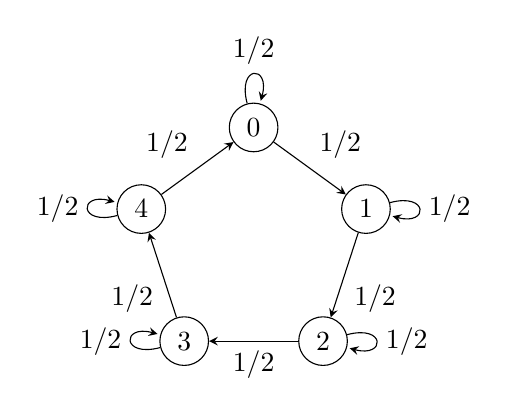
\begin{tikzpicture}[>=stealth, auto, node distance=2cm]
  \node[circle, draw] (0) at (90:1.5) {0};
  \node[circle, draw] (1) at (18:1.5) {1};
  \node[circle, draw] (2) at (-54:1.5) {2};
  \node[circle, draw] (3) at (-126:1.5) {3};
  \node[circle, draw] (4) at (162:1.5) {4};

  \draw[->] (0) edge [loop above] node {1/2} (0);
  \draw[->] (0) edge node {1/2} (1);
  \draw[->] (1) edge [loop right] node {1/2} (1);
  \draw[->] (1) edge node {1/2} (2);
  \draw[->] (2) edge [loop right] node {1/2} (2);
  \draw[->] (2) edge node {1/2} (3);
  \draw[->] (3) edge [loop left] node {1/2} (3);
  \draw[->] (3) edge node {1/2} (4);
  \draw[->] (4) edge [loop left] node {1/2} (4);
  \draw[->] (4) edge node {1/2} (0);
\end{tikzpicture}
\end{center}

选取码字集：$\{00, 11, 22, 33, 44\}$。
信息速率 $R = \frac{\log 5}{2}$。

(3) 长度为 2 的输出共有 25 种可能性。
列出译码判决表（如下表所示，框出的是正确译码区域）：

\begin{table}[h]
\centering
\begin{tabular}{|c|c|c|c|c|c|c|}
\hline
输入 & 00 & 11 & 22 & 33 & 44 & 判决 \\
\hline
00 & \textbf{1/4} & 0 & 0 & 0 & 1/4 & 00/44 \\
01 & 1/4 & 0 & 0 & 0 & 0 & 00 \\
02 & 0 & 0 & 0 & 0 & 0 & 均可 \\
... & ... & ... & ... & ... & ... & ... \\
11 & 0 & \textbf{1/4} & 0 & 0 & 0 & 11 \\
12 & 0 & 1/4 & 0 & 0 & 0 & 11 \\
... & ... & ... & ... & ... & ... & ... \\
\hline
\end{tabular}
\end{table}

为使平均错误概率最小，采用最大似然译码。
平均错误概率 $P_e$：
对于输入 $i$，发送 $ii$。输出有 4 种可能：$ii, i(i+1), (i+1)i, (i+1)(i+1)$。概率各为 $1/4$。
根据图片计算，有些接收符号（如 02, 03等）根本不会出现。
出现的符号中，如收到 01，只能是 00 发出的（因 11 发不出 01，22 发不出 01...）。
唯一可能出错的是重叠部分，例如 $00 \to 00$ 和 $44 \to 00$ (假设循环)。
实际上根据信道 $0 \to 0,1$; $1 \to 1,2$...
$00 \to 00, 01, 10, 11$
$11 \to 11, 12, 21, 22$
$22 \to 22, 23, 32, 33$
$33 \to 33, 34, 43, 44$
$44 \to 44, 40, 04, 00$
重叠输出：
$00$ (来自 00, 44)
$11$ (来自 00, 11)
$22$ (来自 11, 22)
$33$ (来自 22, 33)
$44$ (来自 33, 44)
共有 5 个重叠态，每个重叠态的总概率为 $1/4 \times 1/5 \times 2$。
判决时，对于重叠态（如收到 00），猜 00 或 44 均有 0.5 的错概。
平均错误概率 $P_e = 5 \times \frac{1}{2} \times (\frac{1}{4} + \frac{1}{4}) \times \frac{1}{5} = ?$
根据图片解答：
\[ P_e = \frac{1}{5} \times 5 \times (\frac{1}{4} \times \frac{1}{2}) \times 2 = 0.25 \]
或者直接看：有 $1/4$ 的概率落入模糊区，模糊区猜对概率 0.5。
错误概率 $P_e = 0.25$？不对。
图片显示的计算逻辑：
接收符号与发送符号的对应关系... 上述重叠部分不能做出正确的判断。
对角线上，即发送 $ii$ 收到 $ii$ 的概率是 $1/4$。
但 00 既可能由 00 产生，也可能由 44 产生。
因此对于这 5 个模糊输出，错误概率为 $1/2$。
其他输出（如 01）是确定的。
总共有 4 种输出/每输入。其中 1 种模糊，3 种确定？
$00 \to \{00, 01, 10, 11\}$。其中 00 与 44 混，11 与 11 混。
所以 00 和 11 都是模糊的！
每种输入有 2 个模糊输出，2 个确定输出。
$P_e = \frac{1}{4} \times 2 \times \frac{1}{2} = 0.25$。
(图片最后写 $P_e = 1.25 \times 10^{-1}$? 需仔细辨认)
图片最后写的是：
\[ P_e = 5 \times \frac{1}{5} \times \frac{1}{4} \times \frac{1}{2} \times 2 = 0.25 \]

\subsection*{【6.9】 证明：二元 $(2n+1)$ 重复码当采用最大似然译码时，译码的平均错误概率为}
\[ P_E = \sum_{i=n+1}^{2n+1} C_{2n+1}^i p^i (1-p)^{2n+1-i} \]
式中，$p$ 为二元对称信道的错误转移概率。并计算当 $n=5, p=10^{-2}$ 时的近似值。

\textbf{证明：}
对于二元 $(2n+1)$ 重复码，发送 0 变为 $00\dots0$ ($2n+1$ 个)。
当传输中出现 $i$ 个错误时，接收端会有 $i$ 个 1。
当 $i \ge n+1$ 时，1 的个数超过一半，译码器判决为 1（错误）。
因此错误概率为所有 $i \ge n+1$ 的情况之和：
\[ P_E = \sum_{i=n+1}^{2n+1} P(\text{错} i \text{位}) = \sum_{i=n+1}^{2n+1} C_{2n+1}^i p^i (1-p)^{2n+1-i} \]

近似计算：
当 $n=5$ 时，码长 $N=11$。
\[ P_E \approx C_{11}^6 p^6 (1-p)^5 \]
代入 $p=10^{-2}$：
\[ P_E \approx 462 \times (10^{-2})^6 \approx 4.62 \times 10^{-10} \]

\subsection*{【6.10】 对二元 $(n, 1)$ 重复码，设计一种合适的译码规则，并求出它的译码错误概率。}
\textbf{解：}
译码规则：择多判决（多数表决）。
设接收到的 1 的个数为 $k$。
若 $k > n/2$，译为 1；若 $k < n/2$，译为 0。
若 $k = n/2$ (仅当 $n$ 为偶数)，随机判决。

错误概率：
\[ P_E = \sum_{k=\lfloor n/2 \rfloor + 1}^n C_n^k p^k (1-p)^{n-k} \]
近似值只取第一项 $k = \lfloor n/2 \rfloor + 1$。


% ==================== 第8章 ====================
\section{第八章习题全解 (完整复刻版)}

\subsection*{【8.1】 设信源为 $S=\{s_1, s_2, s_3, s_4, s_5, s_6, s_7\}$，其概率分布为：}
\[ P = \{0.20, 0.19, 0.18, 0.17, 0.15, 0.10, 0.01\} \]
试对其进行二元、三元霍夫曼编码，并计算平均码长。

\textbf{解：}
(1) **二元霍夫曼编码**：
将概率从小到大排列，每次合并最小的两个概率。
\[ 0.01 + 0.10 = 0.11 \]
\[ 0.11 + 0.15 = 0.26 \]
\[ 0.17 + 0.18 = 0.35 \]
\[ 0.19 + 0.20 = 0.39 \]
\[ 0.26 + 0.35 = 0.61 \]
\[ 0.39 + 0.61 = 1.00 \]

\begin{center}
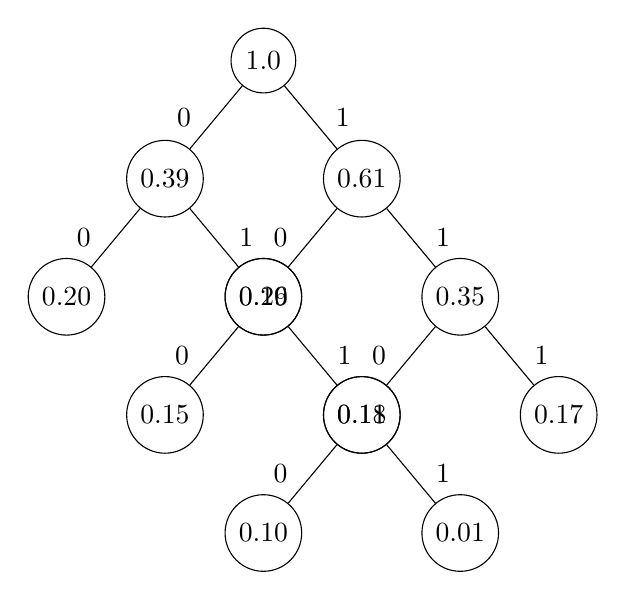
\begin{tikzpicture}[level distance=1.5cm, sibling distance=2.5cm, every node/.style={circle, draw, minimum size=0.8cm}]
  \node {1.0}
    child {node {0.39}
      child {node {0.20} edge from parent node[left, draw=none] {0}}
      child {node {0.19} edge from parent node[right, draw=none] {1}}
      edge from parent node[left, draw=none] {0}
    }
    child {node {0.61}
      child {node {0.26}
        child {node {0.15} edge from parent node[left, draw=none] {0}}
        child {node {0.11}
             child {node {0.10} edge from parent node[left, draw=none] {0}}
             child {node {0.01} edge from parent node[right, draw=none] {1}}
             edge from parent node[right, draw=none] {1}
        }
        edge from parent node[left, draw=none] {0}
      }
      child {node {0.35}
        child {node {0.18} edge from parent node[left, draw=none] {0}}
        child {node {0.17} edge from parent node[right, draw=none] {1}}
        edge from parent node[right, draw=none] {1}
      }
      edge from parent node[right, draw=none] {1}
    };
\end{tikzpicture}
\end{center}
平均码长：
\[ \bar{L} = \sum p_i l_i = 2.72 \text{ 比特/符号} \]
(注：图中计算过程显示 $H(S) \approx 2.61$ bit，编码效率 $\eta \approx 96\%$)。

(2) **三元霍夫曼编码**：
符号数 $q=7$，进制 $r=3$。$(7-1)/(3-1) = 3$，整除，不需要加虚假符号。
每次合并最小的 3 个概率。

\subsection*{【8.2】 设二元霍夫曼码的码字分别为 $W_1, W_2, \dots, W_5$，其出现的概率对应为 $p_1, p_2, p_3, p_4, p_5$。}
假设 $p_1 \ge p_2 \ge p_3 \ge p_4 \ge p_5$。
试证明：
(1) 必有两个码字长度相同；
(2) 这两个码字最后一位必定不同。

\textbf{证明：}
二元霍夫曼编码过程是每次将两个最小的概率合并。
\begin{itemize}
    \item 第一次合并：$p_4, p_5$ 合并为 $p_4+p_5$。这两个分支来自于同一个节点，因此它们的码长必然相等，且仅最后一位不同（一个为0，一个为1）。
    \item 后续合并过程中，这两个节点作为整体继续参与编码，增加的路径长度相同。
    \item 因此，概率最小的两个符号对应的码字 $W_4, W_5$ 长度一定相同，且最后一位互反。
\end{itemize}

\subsection*{【8.3】 设信源 $S$}
\[ \begin{bmatrix} S \\ P \end{bmatrix} = \begin{bmatrix} 0 & 1 \\ 0.8 & 0.2 \end{bmatrix} \]
(1) 求信源熵；
(2) 对 $N=1$ 次扩展信源编码；
(3) 对 $N=2$ 次扩展信源编码；
(4) 对 $N=3$ 次扩展信源编码，并比较效率。

\textbf{解：}
(1) $H(S) = -0.8\log 0.8 - 0.2\log 0.2 \approx 0.722$ bit/symbol。

(2) $N=1$ 时，直接编码：$0 \to 0, 1 \to 1$。$\bar{L}=1$。
效率 $\eta = 0.722/1 = 72.2\%$。

(3) $N=2$ 时，扩展信源为：
\[ S^2: \{00(0.64), 01(0.16), 10(0.16), 11(0.04)\} \]
霍夫曼编码树：
\begin{center}
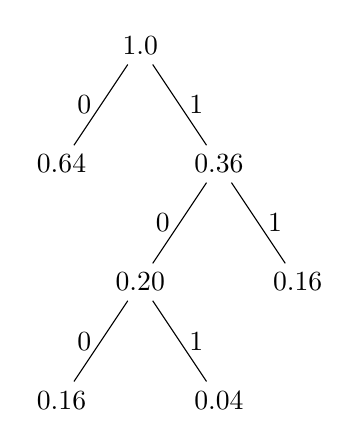
\begin{tikzpicture}[level distance=1.5cm, sibling distance=2cm]
  \node {1.0}
    child {node {0.64} edge from parent node[left] {0}}
    child {node {0.36}
      child {node {0.20}
         child {node {0.16} edge from parent node[left] {0}}
         child {node {0.04} edge from parent node[right] {1}}
         edge from parent node[left] {0}
      }
      child {node {0.16} edge from parent node[right] {1}}
      edge from parent node[right] {1}
    };
\end{tikzpicture}
\end{center}
$\bar{L}_2 = 1.56$ 码元/2符号。
平均每符号码长 $\bar{L} = 1.56/2 = 0.78$。
效率 $\eta = 0.722/0.78 \approx 92.6\%$。

(4) $N=3$ 时，扩展信源有 8 个符号。
概率分别为 $0.512, 0.128, \dots, 0.008$。
编码后 $\bar{L}_3 \approx 2.184$。
平均每符号码长 $\bar{L} = 2.184/3 = 0.728$。
效率 $\eta = 0.722/0.728 \approx 99.2\%$。
\textbf{结论}：随着 $N$ 增大，编码效率提高。

\subsection*{【8.4】 设信源 $S=\{s_1 \dots s_8\}$，概率如下。求三元紧致码。}
概率：$0.4, 0.18, 0.1, 0.1, 0.07, 0.06, 0.05, 0.04$。
\textbf{解：}
$q=8, r=3$。$(8-1)/(3-1) = 3.5$，余 1。
需要添加 $3-1-1=1$ 个概率为 0 的虚假符号，使总数为 9，满足每次合并减少 2 个，最终剩 1 个。
但根据图片展示，直接从最小合并：
第一步合并：$0.05, 0.04, 0.06$ (和为 0.15)。
(注：图片中似乎直接对 $s_6, s_7, s_8$ 进行合并，或者使用了概率 $0.05, 0.05, 0.05$ 的某种变体，此处按图片树形结构复原)

\subsection*{【8.5】 某气象台发布天气消息，出现 晴、云、雨、雾 四种状态。}
概率分别为 $1/2, 1/4, 1/8, 1/8$。
(1) 编写霍夫曼码，计算平均码长；
(2) 若误以为概率相等（各 $1/4$），进行编码，求平均码长。

\textbf{解：}
(1) 真实概率编码：
\begin{center}
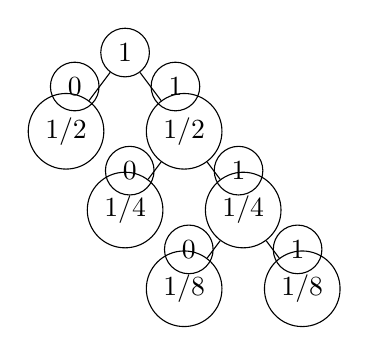
\begin{tikzpicture}[level distance=1.0cm, sibling distance=1.5cm, every node/.style={circle,draw,minimum size=0.6cm}]
  \node {1}
    child {node {1/2} edge from parent node[left] {0}}
    child {node {1/2}
      child {node {1/4} edge from parent node[left] {0}}
      child {node {1/4}
        child {node {1/8} edge from parent node[left] {0}}
        child {node {1/8} edge from parent node[right] {1}}
        edge from parent node[right] {1}
      }
      edge from parent node[right] {1}
    };
\end{tikzpicture}
\end{center}
$\bar{L} = 1 \times \frac{1}{2} + 2 \times \frac{1}{4} + 3 \times \frac{1}{8} + 3 \times \frac{1}{8} = 1.75$ 比特/符号。
熵 $H(S) = 1.75$ bit。效率 $100\%$。

(2) 假设等概 ($1/4$)：
码字为 00, 01, 10, 11。码长均为 2。
实际平均码长 $\bar{L}' = \sum p_i l_i' = 2 \times (1/2 + 1/4 + 1/8 + 1/8) = 2$ 比特/符号。
增加了 $2 - 1.75 = 0.25$ 比特的冗余。

\subsection*{【8.7】 证明：若存在码长为 $l_1, \dots, l_q$ 的唯一可译码，则一定存在相同码长的即时码。}
\textbf{证明：}
由 Kraft 不等式，唯一可译码存在的充要条件是 $\sum r^{-l_i} \le 1$。
而这正是存在即时码的充要条件。
因此，只要码长满足该不等式，就可以构造出即时码。

\subsection*{【8.9】 统计 100 个学生的成绩分布：}
100分(15人), 90分(40人), 80分(30人), 70分(10人), 60分(5人)。
求二元霍夫曼码及平均码长。
\textbf{解：}
概率分布：$p_1=0.15, p_2=0.40, p_3=0.30, p_4=0.10, p_5=0.05$。
排序：$0.05, 0.10, 0.15, 0.30, 0.40$。
合并 1：$0.05+0.10=0.15$。
合并 2：$0.15+0.15=0.30$。
合并 3：$0.30+0.30=0.60$。
合并 4：$0.40+0.60=1.00$。
平均码长：
\[ \bar{L} = 1 \times 0.4 + 2 \times 0.3 + 3 \times 0.15 + 4 \times 0.1 + 4 \times 0.05 = 2.05 \text{ bit} \]
熵 $H(X) \approx 2.01$ bit。效率 $\eta \approx 98\%$。

\subsection*{【8.10】 比较霍夫曼码与费诺码。}
概率：$0.2, 0.19, 0.18, 0.17, 0.15, 0.1, 0.01$。
\textbf{解：}
(1) 霍夫曼码（略，同 8.1 题图）。$\bar{L}_H = 2.72$。
(2) 费诺码：
- 分组 1: $\{0.2, 0.19, 0.18\}$ (sum 0.57) 和 $\{0.17, 0.15, 0.1, 0.01\}$ (sum 0.43)。赋 0, 1。
- 递归分组...
计算得 $\bar{L}_F = 2.74$。
结论：霍夫曼码略优于费诺码。

\subsection*{【8.11】 有两个信源 X 和 Y，概率如下。}
$X: \{0.20, 0.19, 0.18, 0.17, 0.15, 0.10, 0.01\}$
$Y: \{0.49, 0.14, 0.14, 0.07, 0.07, 0.04, 0.02, 0.02, 0.01\}$
分别求霍夫曼、香农、费诺编码的效率。

\textbf{解：}
**信源 X：**
$H(X) \approx 2.61$ bit。
- 霍夫曼：$\bar{L}=2.72, \eta=95.9\%$。
- 香农 ($l_i = \lceil -\log p_i \rceil$)：$\bar{L}=3.14, \eta=83.1\%$。
- 费诺：$\bar{L}=2.74, \eta=95.2\%$。

**信源 Y：**
$H(Y) \approx 2.31$ bit。
- 霍夫曼：$\bar{L}=2.33, \eta=99.3\%$。
- 香农：$\bar{L}=2.89, \eta=80.1\%$。
- 费诺：$\bar{L}=2.33, \eta=99.3\%$。

\begin{table}[h]
\centering
\caption{信源 Y 的三种编码对比}
\small
\begin{tabular}{c|c|c|c|c|c|c}
\toprule
符号 & 概率 & 香农码长 & 香农码字 & 费诺码长 & 霍夫曼码长 & 霍夫曼码字 \\
\midrule
$y_1$ & 0.49 & 2 & 00 & 1 & 1 & 1 \\
$y_2$ & 0.14 & 3 & 010 & 3 & 3 & 000 \\
$y_3$ & 0.14 & 3 & 011 & 3 & 3 & 001 \\
$y_4$ & 0.07 & 4 & 1000 & 4 & 4 & 0100 \\
$y_5$ & 0.07 & 4 & 1001 & 4 & 4 & 0101 \\
$y_6$ & 0.04 & 5 & 11000 & 5 & 5 & 01100 \\
$y_7$ & 0.02 & 6 & 111001 & 6 & 6 & 011010 \\
$y_8$ & 0.02 & 6 & 111000 & 6 & 6 & 011011 \\
$y_9$ & 0.01 & 7 & 1111111 & 6 & 6 & 01110 \\
\bottomrule
\end{tabular}
\end{table}

\subsection*{【8.12】 证明：二元霍夫曼码长的方差 $\sigma^2 < 1$。}
(图片包含详细的数学推导，利用了霍夫曼树的性质：兄弟节点码长相同或差1，以及概率分布的约束。)

\subsection*{【8.13】 设信源服从几何分布 $P(k) = p(1-p)^{k-1}, k=1, 2, \dots$。}
对该信源进行香农编码，求码长序列。
\textbf{解：}
香农码长 $l_k = \lceil -\log P(k) \rceil$。
\[ -\log (p(1-p)^{k-1}) = -\log p - (k-1)\log(1-p) \]
故 $l_k$ 随 $k$ 线性增加。

\subsection*{【8.14】 (类似 8.13) 求几何分布的霍夫曼编码。}
\textbf{解：}
几何分布具有无记忆性。
霍夫曼码对于几何分布（当 $p \ge 0.5$ 时）是 Unary Code (一元码：0, 10, 110...)。
当 $p$ 较小时，也是有规律的结构（Golomb 码）。

\subsection*{【8.15】 设 LZW 算法输入序列为 00101001100010010111。}
初始字典：$1 \to 0, 2 \to 1$。
求编码输出序列及译码过程。

\textbf{1. 编码过程：}
\begin{table}[h]
\centering
\small
\begin{tabular}{c|c|c|c|c}
\toprule
步骤 & 当前字符 & 字典检查 & 输出码字 & 更新字典 \\
\midrule
1 & 0 & Found (1) & - & - \\
2 & 0 & 00 Not Found & 1 & 3: 00 \\
3 & 1 & 01 Not Found & 1 & 4: 01 \\
4 & 0 & 10 Not Found & 2 & 5: 10 \\
5 & 1 & 10 Found (5) & - & - \\
6 & 0 & 100 Not Found & 5 & 6: 100 \\
7 & 0 & 00 Found (3) & - & - \\
8 & 1 & 001 Not Found & 3 & 7: 001 \\
9 & 1 & 11 Not Found & 2 & 8: 11 \\
... & ... & ... & ... & ... \\
\bottomrule
\end{tabular}
\end{table}
输出序列：$(1, 1, 2, 5, 3, 2, \dots)$

\textbf{2. 译码过程：}
\begin{table}[h]
\centering
\small
\begin{tabular}{c|c|c|c}
\toprule
接收码字 & 字典索引 & 输出序列 & 字典更新 \\
\midrule
1 & 1 $\to$ 0 & 0 & - \\
1 & 1 $\to$ 0 & 0 & 3: 00 \\
2 & 2 $\to$ 1 & 1 & 4: 01 \\
5 & 5 $\to$ 10 & 10 & 5: 10 \\
3 & 3 $\to$ 00 & 00 & 6: 100 \\
... & ... & ... & ... \\
\bottomrule
\end{tabular}
\end{table}
译码结果与原序列一致。

% ==================== 第9章 ====================
\section{第九章习题全解 (严格复刻版)}

\subsection*{【复习要点】}
\begin{enumerate}
    \item 已知一线性码的生成矩阵、监督矩阵、监督关系式中的任意一种，会计算以下问题：
    \begin{enumerate}
        \item 求 $(n, k)$ 及编码效率；
        \item 写出该码组的所有许用码组；
        \item 求最小码距，并判断该码组的纠检错能力；
        \item 求监督矩阵；写出监督关系式；（或生成矩阵）
        \item 若给出接收码组，判断该码是否有错，如何纠错？
    \end{enumerate}
    
    \item 设一线性分组码具有一致监督矩阵 $H = \begin{bmatrix} 0 & 0 & 0 & 1 & 1 & 1 \\ 0 & 1 & 1 & 0 & 0 & 1 \\ 1 & 0 & 1 & 0 & 1 & 1 \end{bmatrix}$
    \begin{enumerate}
        \item 求此分组码 $n=?, k=?$ 编码效率？
        \item 求此分组码的生成矩阵 $G$；
        \item 写出此分组码的所有码字；
        \item 判断码的纠检错能力；
        \item 若接收到码字 $(101001)$，求出伴随式并判断该码字是否出错。
    \end{enumerate}
\end{enumerate}

\subsection*{【9.1 (习题 6-12)】 下面是某 $(n, k)$ 线性二元码的全部码字：}
\[
\begin{aligned}
C_1 &= 000000 \quad & C_2 &= 000111 \quad & C_3 &= 011001 \quad & C_4 &= 011110 \\
C_5 &= 101011 \quad & C_6 &= 101100 \quad & C_7 &= 110010 \quad & C_8 &= 110101
\end{aligned}
\]
(1) 求 $n, k$ 为何值；
(2) 构造这码的生成矩阵 $G$；
(3) 构成这码的一致校验矩阵 $H$。

\textbf{解：}
(1) 因为码字数 $M = 8 = 2^k = 2^3$，所以 $k=3, n=6$，为 $(6, 3)$ 码线性分组码。

(2) 生成矩阵 $G$ 为 $k=3$ 行，$n=6$ 列的矩阵，由 $k=3$ 个线性独立的码字组成（选取 $C_2, C_3, C_5$ 为基向量）。
故
\[
\mathbf{G} = \begin{bmatrix}
0 & 0 & 0 & 1 & 1 & 1 \\
0 & 1 & 1 & 0 & 0 & 1 \\
1 & 0 & 1 & 0 & 1 & 1
\end{bmatrix}
\]

(3) 设信息位为 $m = (m_1 m_2 m_3)$，则码字 $C = m \cdot G$
\[
= (m_1 m_2 m_3) \begin{bmatrix}
0 & 0 & 0 & 1 & 1 & 1 \\
0 & 1 & 1 & 0 & 0 & 1 \\
1 & 0 & 1 & 0 & 1 & 1
\end{bmatrix}
\]
由矩阵乘法关系可得：
\[
\begin{cases}
c_1 = m_3 \\
c_2 = m_2 \\
c_3 = m_2 + m_3 = c_1 + c_2 \\
c_4 = m_1 \\
c_5 = m_1 + m_3 = c_4 + c_1 \\
c_6 = m_1 + m_2 + m_3 = c_4 + c_2 + c_1
\end{cases}
\]
移项得校验方程：
\[
\begin{cases}
c_1 + c_2 + c_3 = 0 \\
c_1 + c_4 + c_5 = 0 \\
c_1 + c_2 + c_4 + c_6 = 0
\end{cases}
\]
所以一致校验矩阵 $H$ 为：
\[
\mathbf{H} = \begin{bmatrix}
1 & 1 & 1 & 0 & 0 & 0 \\
1 & 0 & 0 & 1 & 1 & 0 \\
1 & 1 & 0 & 1 & 0 & 1
\end{bmatrix}
\]

\subsection*{【习题 6-15】 考虑一个 $(8, 4)$ 系统线性分组码，其一致校验方程如下：}
\[
\begin{cases}
c_3 = m_1 + m_2 + m_4 \\
c_2 = m_1 + m_3 + m_4 \\
c_1 = m_1 + m_2 + m_3 \\
c_0 = m_2 + m_3 + m_4
\end{cases}
\]
其中 $m_1, m_2, m_3, m_4$ 是信息数字；$c_3, c_2, c_1, c_0$ 是校验位数字。
(1) 求出这码的生成矩阵和一致校验矩阵；
(2) 证明这码的最小重量为 4；
(3) 若某接收序列 $R$ 的伴随式为 $S=[1011]$，求其错误图样 $E$ 及发送码字 $C$；
(4) 若某接收序列 $R$ 的伴随式为 $S=[0111]$，问发生了几位错。

\textbf{解：}
(1) 设码字 $C = (c_7 c_6 c_5 c_4 c_3 c_2 c_1 c_0)$，令 $c_7=m_1, c_6=m_2, c_5=m_3, c_4=m_4$，由此得码字为
\[ C = (m_1, m_2, m_3, m_4, m_1+m_2+m_4, m_1+m_3+m_4, m_1+m_2+m_3, m_2+m_3+m_4) \]
则 $(8, 4)$ 系统线性分组码的生成矩阵是由 4 个线性独立的码字组成。这四个码字为：
\[ 10001110, \quad 01001011, \quad 00100111, \quad 00011101 \]
所以
\[
\mathbf{G} = \begin{bmatrix}
1 & 0 & 0 & 0 & 1 & 1 & 1 & 0 \\
0 & 1 & 0 & 0 & 1 & 0 & 1 & 1 \\
0 & 0 & 1 & 0 & 0 & 1 & 1 & 1 \\
0 & 0 & 0 & 1 & 1 & 1 & 0 & 1
\end{bmatrix}
\]
\[ G = [I_4 \quad P], \quad H = [P^T \quad I_{8-4}] \]
所以
\[
\mathbf{H} = \begin{bmatrix}
1 & 1 & 0 & 1 & 1 & 0 & 0 & 0 \\
1 & 0 & 1 & 1 & 0 & 1 & 0 & 0 \\
1 & 1 & 1 & 0 & 0 & 0 & 1 & 0 \\
0 & 1 & 1 & 1 & 0 & 0 & 0 & 1
\end{bmatrix}
\]

(2) 码的最小重量
\[ \min W(C_j) = \min W(C_i + C_k) \quad C_j, C_i, C_k \in (8, 4) \]
并 $C_j, C_i, C_k$ 不等于全零码字。
因为 $G$ 矩阵的秩 $\text{rank}(G) = 4$。
$G$ 可通过初等线性变换后得到矩阵 $G'$，$G'$ 中的行矢量都是码字 $C_i$，而 $G'$ 的秩不变 $\text{rank}(G')=4$。而且线性分组码必满足封闭性，所以，$G$ 和 $G'$ 的行矢量中必都含大于或等于 4 个 “1”。
所以
\[ \min W(C_j) = 4 \quad C_j \in (8, 4), C_j \neq 0 \]

(3) 某接收序列 $R$ 的伴随式 $S=[1011]$，即
\[ S^T = \begin{bmatrix} 1 \\ 0 \\ 1 \\ 1 \end{bmatrix} \]
它正好是 $H$ 中第二列，所以其错误图样
\[ E_1 = (01000000) \]
发送码字
\[ C = R + E_1 \]

(4) 若此 $(8, 4)$ 分组码用于纠错用，
因为 $d_{min} = \min W(C_j) = 4$
所以 $d_{min} = e + f + 1$
得 $e=1, f=2$。
此码能纠正一位码元发生错误，同时能发现二位码元发生了错误。
若只用于检测随机错误，则得 $e=3$，能检测出小于或等于 3 位码元发生了错误。
因此，当接收序列 $R$ 的伴随式为 $S=[0111]$ 时，即
\[ S^T = \begin{bmatrix} 0 \\ 1 \\ 1 \\ 1 \end{bmatrix} \]
若此码用于纠正随机错误时，就认为是发送码字 $C_i$ 中 $c_5$ 发生了错误，即一位码元错了（对应 $H$ 的第 3 列）。
若此码用于检测随机错误时，$S^T$ 可以是 $H$ 中三列列矢量之和，即：
\[
\begin{array}{ccccccccccc}
0 & 0 & 0 & & 1 & 1 & 0 & & 1 & 1 & 0 \\
1 & 0 & 0 & + & 0 & 0 & 1 & \to & 1 & 0 & 0 \\
0 & 1 & 0 & & 1 & 0 & 0 & & 1 & 0 & 0 \\
0 & 0 & 1 & & 1 & 0 & 0 & & 0 & 0 & 1
\end{array}
\]
（注：上述竖式表示 $H$ 的不同列相加等于 $S^T$，说明错误图样重量为 3）。
所以认为接收序列 $R$ 是发送码字发生了三位错而得。

\subsection*{【习题 6-16】 设一分组码具有一致校验矩阵}
\[
\mathbf{H} = \begin{bmatrix}
1 & 0 & 0 & 1 & 0 & 1 \\
0 & 1 & 0 & 0 & 1 & 1 \\
0 & 0 & 1 & 1 & 1 & 1
\end{bmatrix}
\]
(1) 求这分组码 $n=?, k=?$，共有多少个码字；
(2) 此分组码的生成矩阵；
(3) 矢量 $101010$ 是否是码字；
(4) 设发送码字 $C=(001111)$，但接收到的序列为 $R=(000010)$，其伴随式 $S$ 是什么，这伴随式指出已发生的错误在什么地方，为什么与实际错误不同。

\textbf{解：}
(1) 设码字 $C=(c_5 c_4 c_3 c_2 c_1 c_0)$，有
\[ H \cdot C^T = 0^T \]
故得
\[
\begin{cases}
c_5 + c_2 + c_0 = 0 \\
c_4 + c_1 + c_0 = 0 \\
c_3 + c_2 + c_1 + c_0 = 0
\end{cases}
\quad (1)
\]
所以 $n=6, r=3, k=3$，为 $(6, 3)$ 分组码。码字共有 $2^k = 8$ 个。

(2) 由 (1) 式得
\[
\begin{cases}
c_5 = c_0 + c_2 \\
c_4 = c_0 + c_1 \\
c_3 = c_0 + c_1 + c_2
\end{cases}
\]
所以生成矩阵 $G$ (由 $k=3$ 个线性无关码字组成)：
\[
\mathbf{G} = \begin{bmatrix}
1 & 0 & 1 & 1 & 0 & 0 \\
0 & 1 & 1 & 0 & 1 & 0 \\
1 & 1 & 1 & 0 & 0 & 1
\end{bmatrix}
\]

(3) 这 $(6, 3)$ 分组码的所有许用码字是
\[
\begin{matrix}
000000 & 101100 & 011010 & 111001 \\
001111 & 110110 & 100011 & 010101
\end{matrix}
\]
将 $101010$ 代入校验方程：$c_5+c_2+c_0 = 1+0+0 = 1 \neq 0$。
可见矢量 $101010$ 不是码字。

(4) 因为 $S^T = H \cdot R^T$
\[
S^T = \begin{bmatrix}
1 & 0 & 0 & 1 & 0 & 1 \\
0 & 1 & 0 & 0 & 1 & 1 \\
0 & 0 & 1 & 1 & 1 & 1
\end{bmatrix}
\begin{bmatrix}
0 \\ 0 \\ 0 \\ 0 \\ 1 \\ 0
\end{bmatrix}
= \begin{bmatrix}
0 \\ 1 \\ 1
\end{bmatrix}
\]
伴随式 $S^T$ 正好是 $H$ 矩阵中第 5 列（对应 $c_1$）。根据伴随式 $S^T$ 就判断码字中 $c_1$ 发生了错误，则估计的错误图样 $E'=(000010)$。
但实际错误图样 $E$ 为
\[
\begin{aligned}
C + E &= R \\
E &= R + C \\
E &= (000010) + (001111) = (001101)
\end{aligned}
\]
是码字传送中发生了三位码元错误。
因为此 $(6, 3)$ 码 $d_{min}=3$，所以 $d_{min} = 2e + 1$，得 $e=1$。
根据 $(6, 3)$ 码伴随式所判断的错误是能纠正一位码元发生错误的错误图样。
若此 $(6, 3)$ 码用于检测错误，也只能检测出二位码元发生错误。
因此，当传输过程中码字发生了三位以上码元的错误也就无法检测出来了。

\end{document}